\input{/Users/daniel/github/config/preamble.sty}
\input{/Users/daniel/github/config/ops.sty}

\makeatletter%Instead of bigwedge
\newcommand{\extp}{\@ifnextchar^\@extp{\@extp^{\,}}}
\def\@extp^#1{\mathop{\bigwedge\nolimits^{\!#1}}}
\makeatother

\usepackage[style=authortitle-terse,backend=bibtex]{biblatex}
\addbibresource{complex-geometry.bib}

\begin{document}
{\Huge complex geometry}
\tableofcontents

\section{abstract nonsense}
\begin{defn}\leavevmode
	\begin{itemize}
		\item A \textbf{\textit{pullback}} of the morphisms $f$ and $g$ consists of an object $P$ and two morphisms $p_1:P\to X$ and $p_2:P\to Y$ satisfying the following universal property:
		\[\begin{tikzcd}
			Q\arrow[rrd,bend left,"q_2"]\arrow[ddr,"q_1",swap,bend right]\arrow[dr,dashed,"\phi"]\\
			&P\arrow[r,"p_2"] \arrow[rd, phantom, "\lrcorner", very near start]\arrow[d,"p_1",swap]&Y\arrow[d,"g"]\\
			&X\arrow[r,"f",swap]&Z
		\end{tikzcd}\]
		\item A \textbf{\textit{pushout}} of the morphisms $f$ and $g$ consists of an object $P$ and two morphisms $i_1:P\to X$ and $i_2:P\to Y$ satisfying the following universal property:
		\[\begin{tikzcd}
			Z\arrow[r,"g"]\arrow[d,swap,"f"]&Y\arrow[d,"i_2"]\arrow[ddr,bend left,"j_2"]\\
			X\arrow[r,"i_1",swap]\arrow[drr,bend right,swap,"j_1"]&P\arrow[ul, phantom, "\ulcorner", very near start]\arrow[dr,dashed,"\phi"]\\
			&&Q
		\end{tikzcd}\]
		\item A \textbf{\textit{product}} of $X$ and $Y$ is an object $X\sqcup Y$ and a pair of morphisms $p_1:X\sqcap Y\to X$, $p_2:X\sqcap Y\to Y$ satisfying the following universal property:
		\[\begin{tikzcd}
			Q\arrow[rrd,bend left,"q_2"]\arrow[ddr,"q_1",swap,bend right]\arrow[dr,dashed,"\phi"]\\
			&X\sqcap Y\arrow[r,"p_2"]\arrow[d,"p_1",swap]&Y\\
			&X
		\end{tikzcd}\]
		\item A \textbf{\textit{coproduct}} of $X$ and $Y$ is an object $X\sqcup Y$ and a pair of morphisms $i_1:X\to X\sqcup Y$, $i_2:Y\to X\sqcup Y$ satisfying the following universal property:
		\[\begin{tikzcd}
			&Y\arrow[d,"i_2"]\arrow[ddr,bend left,"j_2"]\\
			X\arrow[r,"i_1",swap]\arrow[drr,bend right,swap,"j_1"]&X\sqcup Y\arrow[dr,dashed,"\phi"]\\
			&&Q
		\end{tikzcd}\]
		\item A morphism $i$ has the \textbf{\textit{left lifting property with respect to a morphism $p$}} and $p$ has the \textbf{\textit{right lifting property with respect to $i$}} if for each morphisms $f$ and $g$, if the outer square in the following diagram commutes, there exists $\phi$ (I think not necessarily unique) completing the diagram:
		\[\begin{tikzcd}[row sep=large]
			A\arrow[r,"f"]\arrow[d,"i",swap]&X\arrow[d,"p"]\\
			B\arrow[r,"g",swap]\arrow[ur,dashed,"\phi"]&Y
		\end{tikzcd}\]
		\item The \textbf{\textit{kernel}} of a morphism is that part of its domain which is sent to zero. Formally, in a category with an initial object 0 and pullbacks, the \textbf{\textit{kernel $\ker f$}} of a morphism $f:A\to B$ is the pullback $\ker(f)\to A$ along $f$ of the unique morphism $0\to B$
		
		More explicitly, this characterizes the object $\ker(f)$ as \textit{the} object (unique up to isomorphism) that satisfies the following universal property:
		\begin{quote}
			for every object $C$ and every morphism $h:C\to A$ such that $f\circ h=0$ is the zero morphism, there is a unique morphism $\phi:C\to\ker(f)$ such that $h=p\circ\phi$.
		\end{quote}
		\[\begin{tikzcd}
			C\arrow[dr,dashed,"\phi"]\arrow[ddr,bend right,swap,"h"]\\
			&\ker(f)\arrow[d]\arrow[r]&0\arrow[d]\\
			&A\arrow[r,"f",swap]&B\arrow[ul, phantom, "\ulcorner", very near start]
		\end{tikzcd}\]
		\item In a category with a terminal object 1, the \textbf{\textit{cokernel}} of a morphism $f:A\to B$ is the pushout (arrows $h$ and $\phi$ apply if terminal object is zero)
		\[\operatorname{coker}(f):=1\sqcup_AB\qquad\qquad\begin{tikzcd}
			A\arrow[r,"f"]\arrow[d]\arrow[dr, phantom, "\lrcorner", very near start]&B\arrow[d]\arrow[rdd,bend left,"h"]\\
			1\arrow[r]&\operatorname{coker}(f)\arrow[dr,dashed,"\phi"]\\
			&&C
		\end{tikzcd}\]
		In the case when the terminal object is in fact zero object, one can, more explicitly, characterize the object $\operatorname{coker}(f)$ with the following universal property:
		\begin{quote}
			for every object $C$ and every morphism $h:B\to C$ such that $h\circ f=0$ is the zero morphism, there is a unique morphism $\phi:\operatorname{coker}(f)\to C$ such that $h=\phi\circ i$.
		\end{quote}
		
		\item A morphism $f:X\to Y$ is a \textbf{\textit{monomorphism}} if for every object $Z$ and every pair of morphisms $g_1,g_2:Z\to X$ then
		\[f\circ g_1=f\circ g_2\implies g_1=g_2.\]
		\[\begin{tikzcd}
			Z\arrow[r,shift={(0,.06)},"g_1"]\arrow[r,swap,shift={(0,-.06)},"g_2"]\arrow[rr,bend left,"f\circ g_1"]\arrow[rr,bend right,swap,"f\circ g_2"]&X\arrow[r,"f"]&Y
		\end{tikzcd}\]
		Equivalently, $f$ is a monomorphism if for every $Z$ the hom-functor $\Hom(Z,-)$ takes it to an injective function
		\[\begin{tikzcd}
			\Hom(Z,X)\arrow[r,hook,"f_*"]&\Hom(Z,Y).
		\end{tikzcd}\]
		Being a monomorphism in a category $\Cc$ means equivalently that it is an epimorphism in the opposite category $\Cc^{\op}$.
		
		\item A morphism $f:X\to Y$ is a \textbf{\textit{epimorphism}} if for every object $Z$ and every pair of morphisms $g_1,g_2:Y\to Z$ then
		\[g_1\circ f=g_2\circ f\implies g_1=g_2.\]
		\[\begin{tikzcd}
			X\arrow[r,"f"]\arrow[rr,bend right,swap,"g_2\circ f"]\arrow[rr,bend left,"g_1\circ f"]&Y\arrow[r,shift={(0,.06)},"g_1"]\arrow[r,swap,shift={(0,-.06)},"g_2"]&Z
		\end{tikzcd}\]
		Equivalently, $f$ is a epimorphism if for every $Z$ the hom-functor $\Hom(-,Z)$ takes it to an injective function
		\[\begin{tikzcd}
			\Hom(Y,Z)\arrow[r,hook,"f^*"]&\Hom(X,Z).
		\end{tikzcd}\]
		Being a monomorphism in a category $\Cc$ means equivalently that it is an monomorphism in the opposite category $\Cc^{\op}$.
	\end{itemize}
\end{defn}
\section{sheaf cohomology}
Let's read \cite{huybrechts}, appendix B.

In the following, $M$ will be a topological space. In most of the examples it is a differential or complex manifold.
\begin{defn}
	A \textbf{\textit{pre-sheaf $\Fc$}} of abelian groups (or vector spaces, rings, etc.) on $M$ consists of an abelian group (resp. vecot space, ring, etc.) $\Gamma(U,\Fc)=\Fc(U)$ for every open subset $U\subset M$ and a group homomorphism (resp. linear map, ring homomorphism, etc.) $r_{U,V}:\Fc(V)\to \Fc(U)$ for any two nested open subsets $U\subset V$ satisfying the following two conditions:
	\begin{enumerate}
		\item[$(i)$] $r_{U,U}=\id_{\Fc(U)}$.
		\item[$(ii)$] For open subsets $U\subset V\subset W$ one has $r_{U,V}\circ r_{V,W}=r_{U,V}$.
	\end{enumerate}
	Sometimes, one additionally requires $\Fc(\varnothing)=0$. In order to lighten the notation a bit, one may also write $s|_U$ instead of $r_{U,V}(s)$.
\end{defn}
\begin{example}
	The basic example is $\Fc=\Cc_M^0$, the pre-sheaf of continuous functions on $M$. More precisely, $\Cc_M^0(U)$ is the ring of all continuous maps $f:U\to\R$.
\end{example}
For $\Fc=\Cc_M^0$ one easily verifies the following additional conditions which do not hold for arbitrary pre-sheaves. We let $U=\bigcup U_i$ be the union of open subsets $U_i\subset M$. Then 
\begin{enumerate}
	\item[$(iii)$] If $f,g\in\Cc^0_M\left(\bigcup U_i\right)$ with $r_{U_i,U}(f)=r_{U_i,U}(g)$ for all $i$, then $f=g$.
	\item[$(iv)$] If functions $f_i\in\Cc_M^0(U_i)$ are given for all $i$ such that $r_{U_i\cap U_j,U_i}(f_i)=r_{U_i\cap U_j,U_j}(f_j)$ for any $j$, then there exists a continuous function $f\in\Cc^0_M(U)$ with $r_{U_i,U}(f)=f_i$ for all $i$.
\end{enumerate}
This leads to the definition of a sheaf.

\begin{defn}
	A pre-sheaf $\Fc$ is called a \textbf{\textit{sheaf}} if $(iii)$ and $(iv)$ are satisfied.
\end{defn}
\begin{example}\leavevmode
	\begin{itemize}
		\item The constant pre-sheaf $\R$, for which $\Fc(U)=\R$ for all open subsets $\varnothing\neq U\subset M$ is not a sheaf as soon as $M$ contains a disconnected open subset. So, one works rather with the \textbf{\textit{constant sheaf(!) $\underline{\R}$}}, which, on an open set $U\subset M$ yields the set of all continuous functions $f:U\to\R$, where $\R$ is endowed with the discrete topology.
	
		Of course, one defines in the same manner constant sheaves associated to other vector spaces, groups, rings, etc.
		\item Another important example is the sheaf $\Ec$ of sections of a (topological) vector bundle $\pi:E\to M$. By definition, $\Ec(U)$ is the set of all (continuous) maps $s:U\to E$ with $\pi\circ s=\id_U$.
		
		In fact $\Ec$ is sheaf of $\Cc_M^0$-modules, that is, each $\Ec(U)$ is a $\Cc_M^0(U)$-module and the restriction maps are comparible with the module structures on the different open subsets.
		
		Since the vector bundle $E$ can be recovered from its sheaf of sections $\Ec$, one often uses the same notation $E$ for both.
	\end{itemize}
\end{example}

\begin{defn}
	Let $\Fc$ and $\Gc$ be two (pre-)sheaves. A \textbf{\textit{(pre-)sheaf homomorphism}} $\varphi:\Fc\to\Gc$ is given by group homomorphisms (linear maps, ring homomorphisms, etc.) $\varphi_U:\Fc(U)\to\Gc(U)$ for any open subset $U\subset M$ satisfying $r_{U,V}^{\Gc}\circ \varphi_V=\varphi_U\circ r_{U,V}^{\Fc}$ for any $U\subset V$.
\end{defn}
Once a homomorphism $\varphi:\Fc\to \Gc$ of (pre-)sheaves of abelian groups is given, one constructs the associated pre-sheaves $\ker(\varphi)$, $\img(\varphi)$ and $\operatorname{coker}(\varphi)$ which are defined in the obvious way, that is, $\operatorname{coker}(\varphi)(U)=\operatorname{coker}(\varphi_U:\Fc(U)\to\Gc(U))$.

There is an important subtlety here. If $\varphi$ is a sheaf homomorphism then $\ker(\varphi)$ is a sheaf itself, but $\img(\varphi)$ and $\operatorname{coker}(\varphi)$, in general, are just pre-sheaves. In order to define the cokernel and the image of a sheaf homomorphism as honest sheaves, one needs to introduce the notion of a stalk.
\begin{defn}
	Let $\Fc$ be a (pre-)sheaf on $M$ and $x\in M$. Then the \textbf{\textit{stalk}} of $\Fc$ at $x$ is
	\[\Fc_x:=\{(U,s):x\in U\subset M,s\in\Fc(U)\}/\sim\]
	Here, for two open subsets $U_i$, $i=1,2$ and sections $s_i\in\Fc(U_i)$, $i=1,2$, one sets $(U_1,s_1)\sim(U_2,s_2)$ if there exists an open subset $x\in U\subset U_1\cap U_2$ such that $r_{U,U_1}(s_1)=r_{U,U_2}(s_2)$.
	
	Equivelently, one could introduce the stalk $\Fc_x$ as the direct limit $\Fc_x=\lim_{x\in U}\Fc(U)$.
\end{defn}
\begin{remark}
	One immediatly finds that any section $s\in\Fc(U)$ induces an element $s_x\in\Fc_x$ for any point $x\in U$. Furthermore, any (pre-)sheaf homomorphism $\varphi:\Fc\to\Gc$ induces homomorphisms $\Fc_x\to\Gc_x$ for any $x\in M$.
\end{remark}
\begin{defn}
	The \textbf{\textit{sheaf $\Fc^+$ associated to a pre-sheaf $\Fc$}} is the sheaf for which $\Fc^+(U)$ of an open subset $U\subset M$ is the set of all maps $s:U\to\bigcup_{x\in U}\Fc_x$ with $s(x)\in\Fc_x$ and such that for all $x\in U$ there exists an open subset $x\in V\subset U$ and a section $t\in\Fc(V)$ with $s(y)=t(y)$ for all $y\in V$. {\color{magenta}what?}
\end{defn}
\begin{remark}
	With this definition, $\Fc^+$ is a sheaf and the natural inclusion $\Fc\subset\Fc^+$ is an isomorphism if the pre-sheaf $\Fc$ was already a sheaf. For many constructions one needs to pass from a naturally defined pre-sheaf to its \textbf{\textit{sheafification}}. For example, the tensor product $\Fc\otimes_{\Rc}\Gc$ of two $\Rc$-modules $\Fc$ and $\Gc$ is defined as the sheafification of $U\mapsto\Fc(U)\otimes_{\Rc(U)}\Gc(U)$.
\end{remark}

\begin{defn}
	Let $\varphi:\Fc\to\Gc$ be a homomorphism of sheaves. Then the \textbf{\textit{image sheaf $\img(\varphi)$}} is the sheaf associated with the image pre-sheaf $U\mapsto\img(\varphi_U)$. Analogously, one defines the \textbf{\textit{cokernel sheaf $\operatorname{coker}(\varphi)$}}.
\end{defn}
\begin{defn}
	The sheaf homomorphism $\varphi$ is \textbf{\textit{injective}} if and only if $\ker(\varphi)$ is trivial. Similarly, one says that $\varphi$ is \textbf{\textit{surjective}} if its cokernel sheaf $\operatorname{coker}(\varphi)$ is trivial.
\end{defn}
	The essential difference between the two properties is that $\varphi$ is injective if and only if $\varphi_U$ is injective for any open set $U$. On the other hand, $\varphi$ might be surjective without $\varphi_U$ being surjective for all/any open subset. However, both properties can be detected by ther stalks. More precisely,
\begin{quote}
	$\varphi$ is injective or surjective if and only if $\varphi_x:\Fc_x\to\Gc_x$ is injective respectively surjective for any point $x\in M$.
\end{quote}
\begin{defn}
	A sequence $\Fc^\bullet$ of sheaf homomorphisms
	\[\begin{tikzcd}
		\cdots\arrow[r]&\Fc^i\arrow[r,"\varphi^i"]&\Fc^{i+1}\arrow[r,"\varphi^{i+1}"]&\Fc^{i+2}\arrow[r,"\varphi^{i+2}"]&\cdots
	\end{tikzcd}\]
	is a \textbf{\textit{complex}} if $\varphi^{i+1}\circ\varphi^i=0$ for all $i$. It is in an \textbf{\textit{exact complex}} if $\ker\varphi^{i+1}=\img\varphi^i$ for all $i$.
	
	An exact complex of the form \begin{tikzcd}
		0\arrow[r]&\Fc^0\arrow[r]&\Fc^1\arrow[r]&\Fc^2\arrow[r]&0
	\end{tikzcd} is called \textbf{\textit{short exact sequence}}.
\end{defn}
\begin{coro}
	A complex of the form
	\[\begin{tikzcd}
		0\arrow[r]&\Fc^0\arrow[r]&\Fc^1\arrow[r]&\Fc^2\arrow[r]&0
	\end{tikzcd}\]
	is exact if and only if the induced complex of stalks
	\[ \begin{tikzcd}
		0\arrow[r]&\Fc_x^0\arrow[r]&\Fc_x^1\arrow[r]&\Fc_x^2\arrow[r]&0
	\end{tikzcd}\]
	is exact for any $x\in M$.
\end{coro}
\begin{remark}
	Since surjectivity does not mean surjectivity for any open subset, a short exact sequence as above does not necessarily define short exact sequences
	\[ \begin{tikzcd}
		0\arrow[r]&\Fc^0(U)\arrow[r]&\Fc^1(U)\arrow[r]&\Fc^2(U)\arrow[r]&0
	\end{tikzcd}\]
	for any subset $U\subset M$ and in particular not for $M$. \textbf{This is where cohomology comes in.} It turns out that the failure of surjectivity of $\Fc^1(M)\to\Fc^2(M)$ is measured by the cohomology of $\Fc^0$.
\end{remark}

In order to introduce sheaf cohomology, one has to make a choice. There is the theoretically superior but rather abstract approach via derived categories or the more ad hoc one using acyclic resolutions. We outline the second one.

One first has to single out special sheaves with no cohomology in order to define cohomology for all other ones by resolving them.

\begin{defn}
	A \textbf{\textit{resolution}} of a sheaf $\Fc$ is a complex  
	$\begin{tikzcd}
		0\arrow[r]\mathcal{F}^0\arrow[r]&\mathcal{F}^1\arrow[r]&\Fc^2\arrow[r]&0
	\end{tikzcd}$ together with a homomorphism $\mathcal{F}\to\mathcal{F}^0$ such that
	\[\begin{tikzcd}
		0\arrow[r]&\mathcal{F}\arrow[r]&\mathcal{F}^0\arrow[r]&\mathcal{F}^1\arrow[r]&\mathcal{F}^2\arrow[r]&\cdots
	\end{tikzcd}\]
	is an exact complex of sheaves.
\end{defn}
One possible choice for sheaves without cohomology is provided by flasque sheaves.
\begin{defn}
	A sheaf $\Fc$ is called \textbf{\textit{flasque}} if for any open subset $U\subset M$ the restriction map $r_{U,M}:\mathcal{F}(M)\to\mathcal{F}(U)$ is surjective.
\end{defn}
Why flasque sheaves are the right ones is explained by the following
\begin{lemma}\label{lem:flasque}
	If
	\[\begin{tikzcd}
		0\arrow[r]&\Fc^0\arrow[r]&\Fc^1\arrow[r]&\Fc^2\arrow[r]&0
	\end{tikzcd}\]
	is a short exact sequence and $\Fc^0$ is flasque, then the induced sequence
	\[\begin{tikzcd}
		0\arrow[r]&\Fc^0(U)\arrow[r]&\Fc^1(U)\arrow[r]&\Fc^2(U)\arrow[r]&0
	\end{tikzcd}\]
	is exact for any open subset $U\subset M$.
\end{lemma}
Next, one has to ensure that any sheaf can be resolved by flasque sheaves. This will allow to define the cohomology of any sheaf.
\begin{prop}\label{prop:flasque-resolutions}
	Any sheaf $\Fc$ on $M$ admits a resolution
	\[\begin{tikzcd}
		0\arrow[r]&\Fc\arrow[r]&\Fc^0\arrow[r]&\Fc^1\arrow[r]&\Fc^2\arrow[r]&\cdots
	\end{tikzcd}\]
	such that all sheaves $\Fc^i$, $i=0,1,\ldots$ are flasque.
\end{prop}
\begin{defn}
	The \textbf{\textit{$i$-th cohomology group $H^i(M,\Fc)$}} of a sheaf $\Fc$ is the $i$-th cohomology of the complex
	\[\begin{tikzcd}
		\Fc^0(M)\arrow[r,"\varphi^0"]&\Fc^1(M)\arrow[r,"\varphi^1"]&\Fc^2(M)\arrow[r,"\varphi^2"]&\cdots
	\end{tikzcd}\]
	{\color{cyan}induced by a flasque resolution} $\Fc\to\Fc^\bullet$. Explicitly,
	\[H^i(M,\Fc)=\dfrac{\ker(\varphi^i_M:\Fc^i(M)\to\Fc^{i+1}(M))}{\img(\varphi^{i-1}_M:\Fc^{i-1}(M)\to\Fc^i(M))}\]
\end{defn}
Clearly, with this definition any flasque sheaf $\Fc$ has vanishing cohomology $H^i(M,\Fc)=0$ for $i>0$. (This is because of \cref{lem:flasque}: though it is stated as a \textit{short} exact sequence, it certainly implies exactness at every arrow in a long exact sequence of flasque sheaves.)

Moreover, for any sheaf $\Fc$ one has $\ker\varphi_M^0=H^0(M,\Fc)=\Gamma(M,\Fc)=\Fc(M)$. Indeed, in virtue of \cref{prop:flasque-resolutions}, \[\img(\Fc\to\Fc^0)=\ker(\Fc^0\to\Fc^1)\]
as sheaves, that is, as the sheafifications of the pre-sheaves
\[U\mapsto\img (\varphi_U:\Fc(U)\to\Fc^0(U))\quad \text{and}\quad U\mapsto\ker(\varphi^0_U:\Fc^0(U)\to\Fc^1(U))\]
calling the first arrow $\varphi$ for now. Taking $U=M$, we simply have that
\[\img\varphi_M=\ker\varphi^0_M\]
and $\varphi_M:\Fc(M)\to\Fc^0(M)$ injectively so that $\img\varphi_M\cong\Fc(M)$.

That this definition of cohomology is really independent of the chosen fiasque resolution is due to
\begin{prop}
	If $\Fc\to\Fc^\bullet$ and $\Fc\to\Gc^\bullet$ are two flasque resolutions of a sheaf $\Fc$ then both define naturally isomorphic cohomology groups.
\end{prop}

The most striking feature of cohomology is that it explains fully the non­ exactness of short exact sequences on the level of global sections.
\begin{prop}
	Let
	\[\begin{tikzcd}
		0\arrow[r]&\Fc^0\arrow[r]&\Fc^1\arrow[r]&\Fc^2\arrow[r]&0
	\end{tikzcd}\]
	be a short exact sequence of sheaves on $M$. Then there exists a \textbf{\textit{long exact cohomology sequence}}
	\[\begin{tikzcd}
		0\arrow[r]&H^0(M,\Fc^0)\arrow[r]&H^0(M,\Fc^1)\arrow[r]&H^0(M,\Fc^2)\arrow[dll]\\
		&H^1(M,\Fc^0)\arrow[r]&H^1(M,\Fc^1)\arrow[r]&H^1(M,\Fc^2)\arrow[dll]\\
		&H^2(M,\Fc^0)\arrow[r]&H^2(M,\Fc^1)\arrow[r]&H^2(M,\Fc^2)\arrow[r]&\cdots
	\end{tikzcd}\]
\end{prop}
\begin{defn}
	Suppose $\Fc$ is a sheaf {\color{cyan}of vector spaces} on $M$. Then $h^i(M,\Fc)$ denotes the dimension of $H^i(M,\Fc)$, which inherits a natural vector space structure. If all $h^i(M,\Fc)$ are finite and only finitely many are non-trivial we say $\Fc$ has \textbf{\textit{finite cohomology}} and we define the \textbf{\textit{Euler-Poincaré characteristic of $\Fc$}} as
	\[\chi(M,\Fc):=\sum(-1)^ih^i(M,\Fc).\]
\end{defn}
\begin{remark}
	In \cite{hatcher-at}, we have the following result for a finite CW complex $Y$:
	\[\sum_{i=0}^\infty(-1)^i(\#i-\text{cells})=\sum_{i=0}^\infty(-1)^i\operatorname{ran}H_i(Y;\Z),\]
	where left-hand side is defined as the Euler-Poincaré characteristic $\chi(Y)$.
\end{remark}
\begin{coro}
	Let
	\[\begin{tikzcd}
		0\arrow[r]&\Fc^0\arrow[r]&\Fc^1\arrow[r]&\Fc^2\arrow[r]&0
	\end{tikzcd}\]
	be a short exact sequence of sheaves of vector spaces with finite cohomology. Then
	\[\chi(M,\Fc^1)=\chi(M,\Fc^0)+\chi(M,\Fc^2).\]
\end{coro}
It might happen that flasque resolutions are difficult to find. But in order to compute the cohomology of a sheaf, any resolution by \textbf{\textit{acyclic sheaves}}, i.e. sheaves with trivial higher cohomology groups, can be used. What kind of acyclic sheaves are convenient depends on the situation. For topological, differentiable, and complex manifolds, the following one is very useful. For the Zariski topology one has to use different ones.
\begin{defn}
	A sheaf $\Fc$ is called \textbf{\textit{soft}} is the restriction $\Gamma(M,\Fc)\to\Gamma(K,\Fc)$ is surjective for any closed subset $K\subset M$.
	
	The space of sections $\Gamma(K,\Fc)$ of $\Fc$ over the closed set $K$i\textit{is defined} as the direct limit of the spaces of sections over all open neighbouthoods of $K$.
\end{defn}
\begin{prop}
	Soft sheaves are acyclic. Any sheaf of modules over a soft sheaf of commutative rings is soft and hence acyclic.
\end{prop}
\begin{remark}
	This is frequently applied to the sheaf of continuous (or differentiable) functions on a manifold \textit{which is easily shown to be soft}. Notice that the sheaf of holomorphic functions on a complex manifold \textit{is not soft}.
\end{remark}

\textbf{\textit{\v Chech cohomology}} is another cohomology theory. It has the advantage to be defined without any sheaf resolution. Since it often coincides with the cohomology defined above, we will sketch the main steps of its construction.

Let us first fix an open covering $M=\bigcup_iU_i$ with $I$ an order set and consider the intersections $U_{i_0\ldots i_p}:=U_{i_0}\cap\ldots\cap U_{i_p}$. Then we set
\[C^p(\{U_i\},\Fc)=\prod_{i_0<\ldots<i_p}\Gamma(U_{i_0\ldots i_p},\Fc)\]
{\color{cyan}(It doesn't seem to be a very meaningful definition… I would rather like it if they were formal sums of something like in \cref{remark:chain-complexes})} There is a natural differential
\begin{align*}
	d:C^p(\{U_i\},\Fc)&\to C^{p+1}(\{U_i\},\Fc)\\
	\alpha=\prod\alpha_{i_0\ldots i_p}&\mapsto d\alpha
\end{align*}
with
\[(d\alpha)_{i_0\ldots i_{p+1}}=\sum_{k=0}^{p+1}(-1)^k\alpha_{i_0\ldots\widehat{i_k}\ldots i_{p+1}}|_{U_{i_0\ldots i_p+1}}\]
\begin{remark}\label{remark:chain-complexes}
	Recall from \cite{hatcher-at} that a \textbf{\textit{singular $n$-simplex}} in a space $X$ is by definition just a map $\sigma:\Delta^n\to X$. The word 'singular' is used here to express the idea that $\sigma$ need not be a nice embedding but can have 'singularities' where its image does not look at all like a simplex. All that is required is that $\sigma$ be continuous. Let $C_n(X)$ be the free abelian group with basis the set of singular $n$-simplices in $X$. Elements of $C_n(X)$, called \textbf{\textit{$n$-chains}}, are finite formal sums $\sum_in_i\sigma_i$ for $n_i\in\Z$ and $sigma_i:\Delta^n\to X$. A boundary map $\partial_n:C_n(X)\to C_{n-1}(X)$ is defined by specifying its values on the basis elements:
	\[\partial_n(\sigma)=\sum_i(-1)^i\sigma|[v_0,\ldots,\widehat{v_i},\ldots,v_n],\]
	which intuitively means that the boundary of the $n$-simplex consists of various ordered $(n-1)$-dimensional simplices, where the symbol $\hat{}$ over $v_i$ indicates that this vertex is deleted from the sequence $v_0,\ldots,v_n$.
	
	Then, given a space $X$ and an abelian group $G$, we define the group $C^n(X;G)$ of \textbf{\textit{singular $n$-cochains with coefficients in $G$}} to be the dual group $\Hom(C_n(X),G)$ of the singular chaing group $C_n(X)$. Thus an $n$-cochain $\varphi\in C^n(X;G)$ assigns to each singular $n$-simplex $\sigma:\Delta^n\to X$ a value $\varphi(\sigma)\in G$. Since the singular $n$-simplices form a basis for $C_n(X)$, these values can be chosen arbitrarily, hence $n$-cochains are exactly equivalent to functions from singular $n$-simplices to $G$. A \textbf{\textit{coboundary map}} $\delta:C^n(X;G)\to C^{n+1}(X;G)$ is the dual $\delta^*{\color{cyan}=\Hom(\partial,G)}$, so for a cochain $\varphi\in C^n(X;G)$, its coboundary $\delta\varphi$ is the composition $C_{n+1}(X)\overset{\partial}{\to}C_n(X)\overset{\varphi}{\to}G$.
		\[\begin{tikzcd}
		\textcolor{cyan}{C_{n+1}}\arrow[d,cyan,swap,"\partial"]\arrow[rd,cyan,"\varphi\circ\partial=\partial^*"]\\	\textcolor{cyan}{C_n}\arrow[cyan,swap,r,"\varphi"]&\textcolor{cyan}{G}
	\end{tikzcd}\]
	This means that for a singular $(n+1)$-simplex $\sigma(\Delta^{n+1})\to X$ we have
	\[\varphi\partial (\sigma)=\sum_i(-1)^i\varphi(\sigma|[v_1,\ldots,\widehat{v}_i,\ldots,v_{n+1}])\]
\end{remark}

Back to \cite{huybrechts}, a calculation shows that $d^2=0$, i.e.
\[\begin{tikzcd}
	C^0(\{U_i\},\Fc)\arrow[r,"d"]&C^1(\{U_i\},\Fc)\arrow[r,"d"]&\cdots
\end{tikzcd}\]
is a complex. {\color{magenta}Since $\Fc$ is a sheaf, one finds $\Gamma(M,\Fc)=\ker(d:C^0(\{U_i\},\Fc)\to C^1(\{U_i\},\Fc))$ (I would love to see why…)}.

\begin{defn}
	The \textbf{\textit{$i$-th \v Chech cohomology group}} with respect to the fixed open covering $M=\bigcup_iU_i$ is
	\[\check{H}^i(\{U_i\},\Fc)=\dfrac{\ker(d:C^i(\{U_i\},\Fc)\to C^{i+1}(\{U_i\},\Fc))}{\img(d:C^{i-1}(\{U_i\},\Fc)\to C^i(\{U_i\},\Fc))}\]
	In this way, we have defined cohomology groups without using acyclic sheaves, but which still depend on the open covering $M=\bigcup U_i$. This can be remedied by passing to the limit. More precisely, if $M=\bigcup_i U_i$ is refined by an open covering $M=\bigcup_jV_j$, then there exists a natural map
	\[\check{H}^i(\{U_i\},\Fc)\to\check{H}^i(\{V_j\},\Fc))\]
	and one defines the \v Chech cohomology as a sheaf without specifying an open coveing as
	\[\check{H}^i(M,\Fc):=\lim_\to \check{H}^i(\{U_i\},\Fc).\]
\end{defn}

\subsection{The approach in Donaldson}

Now let's quickly do the approach in \cite{donaldson}.
Consider a topological space $X$ and an open cover $X=\bigcup_\alpha U_\alpha$. For simplicity, suppose $X$ is compact and the cover is finite. The \textbf{\textit{nerve}} if the cover is an abstract simplicial complex with one vertex (a 0-simplex) $\sigma_\alpha$ for every open set $U_\alpha$ and a $p$-simplex $\sigma_{\alpha_0,\ldots,\alpha_p}$ for each non-empty intersection $U_{\alpha_0}\cap\ldots\cap U_{\alpha_p}$. Now, given an abelian group $A$, we can form the simplicial cochain complex of this nerve.

For example, a 0-cochain is the assignment of an element $g_\alpha\in A$ to each $U_\alpha$. A 1-cochain assigns an element $g_{\alpha\beta}\in A$. to each non-empty intersection $U_\alpha\cap U_\beta$ and a 2-cochain assigns an element $g_{\alpha\beta\gamma}$ to each non-empty triple intersection $U_\alpha\cap U_\beta\cap U\gamma$. {\color{cyan}(Now this looks much more like \cref{remark:chain-complexes})} We have cochain groups $C^p$ for $p\geq 0$. There is a standar coboundary map $\delta:C^p\to C^{p+1}$. For example, a 1-cochain $\underline{g}=(a_\alpha)$ has $\delta\underline{g}=\underbrace{h}$ where
\[\underline{h}_{\alpha\beta}=g_\alpha-g_\beta\]
and a 2-cochain $\underline{h}$ has $\delta\underline{h}=\underline{k}$, where
\[\underline{k}_{\alpha\beta\gamma}=h_{\alpha\beta}-h_{\alpha\gamma}+h_{\beta\gamma}\]
{\color{cyan}So this is just a way of writing the definition of the boundary map without writing it. So it's not surprising to have a} \textit{Note:} There is an issue about how one handles orientations here; see any book on algebraic topology.

Now we can form the cohomology of this complex $H^*(X;\Uc,A)$, say, where $\Uc$ denotes the open cover. Suppose $X=\bigcup V_i$ is another cover $\Vc$. We say that $\Vc$ is a \textbf{\textit{refinement}} of $\Uc$ if we can choose a map of index sets $\alpha(i)$ such that $V_i$ is contained in $U_{\alpha(i)}$. In this case, we get a natural induced map on cochain complexes and hence a map $H^*(X;\Uc,A)\to H^*(X;\Vc,A)$. The \textbf{\textit{\v Cech cohomology}} $H^*(X,A)$ of $X$ with co-efficients in $A$ is defined by taking the \textbf{\textit{inverse limit}}:

\begin{quote}
	That is, an element of $H^*(X,A)$ is represented by an alement of $H^*(X;\Uc,A)$ for some cover $\Uc$, but two elements represented by $\omega_1\in H^*(X;\Uc_1,A)$, $\omega_2\in H^*(H;\Uc_2,A)$ are equal in $H^*(X;A)$ if there is some common refinement $\Vc$ of $\Uc_1,\Uc_2$ such that $\omega_1,\omega_2$ have the same image in $H^*(X;\Vc,A)$.
\end{quote}
Thus $H^*(X,A)$ is a topological invariant of $X$ and, at least for reasonable spaces such as manifolds, this is in fact isomorphic to the singular cohomology with coefficients in $A$. In practice, one rarely needs to perfom the limiting process explicitly if one works with a sensible cover.

Now, from this standpoint, the generalisation to ‘sheaf cohomology’ is very easy and natural. To keep things simple, for the moment suppose one has a class $S$ of functions on the space $X$ (these could be continuous functions or, if $X$ is a manifold, smooth functions or, if $X$ is a Riemann surface, holomorphic functions). The only property we require is that for each non-emptu open set $U\subset X$ there is a corresponding set $S(U)$ of functions on $U$ of the given class, and if $U\subset U$ we have a restriction map from $S(U)$ to $S(V)$.

We generalise the \v Cech construction by allowing $g_{\alpha_0,\ldots,\alpha_p}$ to be an element of $S(U_0\cap\ldots\cap U_p)$. The differential $\delta$ is defined by the same formula, but restricting functions on $p+1$ fold intersections to $p$-fold intersections.  Then we get cohomology groups $H^*(X;\Uc,S)$ and, taking limit over coverings, we arrive at an invariant $H^*(X,S)$.

\begin{quote}
	For example, a 0-cochain $\underline{g}$ is given by a function $g_\alpha$ on $U_\alpha$ for each $\alpha$, and the cocycle condition $\delta\underline{g}=0$ asserts that $g_\alpha=g_\beta$ on any non empty intersection $U_\alpha\cap U_\beta$. This just means that the $g_\alpha$ are restrictions of a single function $g$ on $X$. Thus $H^0(X;\Uc,S)=S(X)$.
	
	{\color{cyan}Let us rephrase: a 0-cochain is a formal sum of some holomorphic functions defined on some sets. If this cochain is a cocycle then these functions coincide on the intersections on the sets. Because we are dealing with a sheaf, this means we can make a function on the whole manifold out of the pieces,} {\color{magenta}and then finally I think I am kind of convinced that $H^0(X;\Uc,S)=S(X)$.}
\end{quote}
{\color{cyan}Then we have a discussion on meromorphic functions, definition of a sheaf $\Sc$ on a space $X$, homomorphism of sheaves, injective sheaves, surjective sheaves (which are not what we expect and in fact this is where cohomology came in), and also}
\begin{defn}
	A sheaf $\Sc$ over $M$ is called \textbf{\textit{fine}} if, for each locally finite cover $\{U_i\}$ of $M$ by open sets, there exists for each $i$ an endomorphism $e_i$ of $\Sc$ such that
	\begin{itemize}
		\item $\supp(e_i)\subset U_i$,
		\item $\sum_ie_i=\id$.
	\end{itemize}
	By $\supp$, the \textbf{\textit{support}} of $e_i$ we denote the closure of the set of points $m\in M$ for which $e_i|\Sc_m$ is not zero. We call $\{e_i\}$ a \textbf{\textit{partition of unity}} for $\Sc$ subordinate to the cover $\{U_i\}$ of $M$.
\end{defn}
From our Telegram group (sadly I can't compile the names in Russian…):
\begin{quote}
	\href{https://fr.wikipedia.org/wiki/Faisceau_(mathématiques)#Typologie_des_faisceaux}{Tipologia dos feixes}:
	\begin{itemize}
		\item flabby = flasque
			%=вялый 
			= flácido--- sections extend from open subsets
		\item soft = mou
			%=мягкий 
			= macio--- sections extend from closed subsets
		\item fine = fin
			%=тонкий
	 		= fino--- partition of unity (sheaf of endomorphisms is soft)
	
	And we have:
	
	fine $\implies$ soft $\implies$ flabby $\implies$ acyclic $\implies$ resolutions of this type are useful to compute cohomology
	
	fino $\implies$ macio $\implies$ flácido $\implies$ acíclico $\implies$ útil

	Fine sheaves were introduced by Cartan, flabby and soft by Godement.
	\end{itemize}
\end{quote}

\textbf{Now the basic fact is there is a way to define cohomology groups $H^p(X,\Sc)$ for any sheaf over a space $X$.} Since $X$ is fixed, we will drop it from the notation and just write $H^p(\Sc)$. These can be characterised by the following axioms.
\begin{enumerate}
	\item $H^0(X,\Sc)=\Sc(X)$, the space of \textbf{\textit{global sections}} of $\Sc$.
	\item A sheaf homomorphism $a:\Sc\to\Sc'$ induces homomorphisms from $H^p(X,\Sc)$ to $H^p(X,\Sc')$.
	\item A short exact sequence of sheaves $0\to\Sc\to\Sc'\to\Sc''\to0$ induces a long exact sequence in cohomology
	\[\cdots\to H^p(\Sc')\to H^p(\Sc'')\overset{\delta}{\to}H^{p+1}(\Sc)\to H^{p+1}(\Sc')\to\cdots,\]
	where the boundary maps $\delta$ have an obvious naturality property with respect to homomorphisms of exact sequences.
	\item if $\Sc$ is fine, then $H^p(\Sc)=0$ for $p>0$.
\end{enumerate}

Again from Telegram:
\begin{quote}
	And 'axioms' of Donaldson say merely that $H^p$ are functorial in the sheaf $\Fc$, there is a long exact sequence of cohomology associated with a short exact sequence of sheaves, and fine sheaves are acyclic. First three axioms follow from general formalism of derived functors, fourth gives us a source of sheaves that we can use to construct resolution in order to compute the cohomology (e.g. all sheaves of modules over the sheaf of smooth functions).
\end{quote}

And \cite{donaldson}. One approach is to use the \v Cech construction outlined above to define the groups $H^p(\Sc)$ and then show uniqueness from the axioms. But there are several other approaches, and we refer to more specialised texts for a proper treatment.

\begin{quote}
	{\color{red}\textbf{The point is that however we go about things, we arrive at the same cohomology groups}.}
\end{quote}

Aaaand back to \cite{huybrechts}:
\begin{prop}
	For any open covering $M=\bigcup_iU_i$, there exists an natural homomorphism
	\[\check{H}^i(\{U_i\},\Fc)\to H^i(M,\Fc).\]
\end{prop}
Of course, these homomorphisms are in general not bijective, as the open
covering might be very coarse. However, passing to the limit often results in isomorphism with the true cohomology groups, i.e. when the topological spaces is reasonable (e.g. paracompact), the induced maps $\check{H}^i(M,\Fc)\to H^i(M,\Fc)$ are indeed bijective.
\begin{prop}
	The natural map $\check{H}^1(M,\Fc)\to H^1(M,\Fc)$ is always bijective.
\end{prop}
This opens the way to parametrize line bundles by cohomology classes. Let us sketch this for differentiable real line bundles.

Let $\pi:L\to M$ be a line bundle that can be trivialized over open subsets $U_i$ of an open cover $M=\bigcup U_i$ by maps $\psi_i:L|_{U_i}\cong U_i\times \R$. Then $\{\psi_{ij}:=\psi_i\circ\psi^{-1}_j\in\Cc_M^*(U_i\cap U_j)\}$ {\color{red}can be considered as a cocycle (see \cref{cocycle-condition})} and thus gives rise to an element in $\check{H}^1(\{U_i\},\Cc_M^*)$, where $\Cc^*_M$ is the sheaf of differentiable functions without zeros.

One verifies that this cohomology class does not depend on the choice of the trivializations $\psi_i$. Moreover, any class in $\check{H}^1(\{U_i\},\Cc_M^*)$ can be interpreted as a cocycle of a line bundle trivialized over the open subsets $U_i$.

Thus, by definition every line bundle $L$ gives rise to a cohomology class in the covering independent \v Cech cohomology group $\check{H}^1(M,\Cc^*_M)$ which does not depend neither on the open covering nor on the trivializations. The above proposition then yields

\begin{coro}
	There is a bijection between the set of isomorphism classes of real line bundles on a differentiable manifold $M$ and the group $H^1(M,\Cc^*_M)$.
\end{coro}

{\color{cyan} In sum, since a line bundle can be reconstructed from the gluing maps of the trivializations, and all of those form a cocycle, \textbf{every line bundle is associated to a cocycle!} And it is a bijective correspondence, and that is the Picard group.}

\section{vector bundles}
To make sure we understand that isomorphism let's read some \cite{hatcher-vb}.

\begin{defn}\leavevmode
	\begin{itemize}
		\item An \textbf{\textit{$n$-dimensional vector bundle}} is a map $p:E\to B$ together with a vector space structure on $p^{-1}(b)$ for each $b\in B$ such that the following local triviality condition is satisfied: there is a cover of $B$ by open sets $U_\alpha$ for each of which there exists a homeomorphism $h_\alpha:p^{-1}(U_\alpha)\to U_\alpha\times\R^n$ taking $p^{-1}(b)$ to $\{b\}\times\R^n$ by a vector space isomorphism for each $b\in U_\alpha$. Such an $h_\alpha$ is called a \textbf{\textit{local trivialization}} of the vector bundle. The space $B$ is called the \textbf{\textit{base space}}, $E$ is called the \textbf{\textit{total space}} and the vector spaces $p^{-1}(b)$ are the \textbf{\textit{fibers}}. We could equally well take $\C$ instead of $\R$ to obtain a \textbf{\textit{complex vector bundle}}.
		
		\item An \textbf{\textit{isomorphism}} between vector bundles $p_1:E_1\to B$ and $p_2:E_2\to B$ over the same base space $B$ is a homeomorphism $h:E_1\to E_2$ taking each fiber $p_1^{-1}(b)$ to the corresponding fiber $p_2^{-1}(b)$ by a linear isomorphism.
		
		\item A \textbf{\textit{section}} of a vector bundle $p:E\to B$ is a map $s:B\to E$ assigning to each $b\in B$ a vector $s(b)$ in the fiber $p^{-1}(b)$. The condition $s(b)\in p^{-1}(b)$ can also be written as $ps=\id_B$. Every vector bundle has a canonical section, the \textbf{\textit{zero section}} whose value is the zero vector in each fiber.
		
		\item Given vector bundles $p_1:E_1\to B$ and $p_2:E_2\to B$ over the same base space $B$ we define their \textbf{\textit{direct sum}} to be the space
		\[E_1\oplus E_2=\{(v_1,v_2)\in E_1\times E_2:p_1(v_1)=p_2(v_2)\}.\]
		There is a projection $E_1\oplus E_2\to B$ sending $(v_1,v_2)$ to the point $p_1(v_1)=p_2(v_2)$ making this construction into a vector bundle over $B$.
		
		\item Given vector bundles $p_1:E_1\to B$ and $p_2:E_2\to B$ over the same base space $B$ let $E_1\otimes E_2$, as a set, be the disjoint union of the vector spaces $p_1^{-1}(x)\otimes p_2^{-1}(x)$ for $x\in B$. The topology on this set is defined in the following way. Choose isomorphisms $h_i:p_i^{-1}(U)\to U\times\R^{n_i}$ for each open set $U\subset B$ over which $E_1$ and $E_2$ are trivial. Then the topology $\Tc_U$ on the set $p_1^{-1}(U)\otimes p_2^{-1}(U)$ is defined by letting the fiberwise tensor product map $h_1\otimes h_2:p_1^{-1}(U)\otimes p_2^{-1}(U)\to U\times (\R^{n_1}\otimes\R^{n_2})$ be a homeomorphism.
		
		The toplogy $\Tc_U$ is independent of the choice of the $h_i$'s since any other choices are obtained by composing with isomorphisms of $U\times\R^{n_i}$ of the form $(x,v)\mapsto(x,g_i(x)(v))$ for continuous maps $g_i:U\to \GL_{n_i}(\R)$ {\color{cyan}(this follows from the definition of local trivializations as vector space isomorphisms)}. Hence $h_1\otimes h_2$ changes by composing with analogous isomorphisms of $U\times (\R^{n_1}\otimes\R^{n_2})$ whose second coordinates $g_1\otimes g_2$ are continuous maps $U\to\GL_{n_1n_2}(\R)$, since the entries of the matrices $g_1(x)\otimes g_2(x)$ are the products of the entries of $g_1(x)$ and $g_2(x)$.
		
		When we replace $U$ by an open subset $V$, the topology on $p_1^{-1}(V)\otimes p_2^{-1}(V)$ induced by $\Tc_U$ is the same as the topology $\Tc_V$ since local trivializations over $U$ restrict to local trivializations over $V$. Hence we get a well-defined topology on $E_1\otimes E_2$ making it a vector bundle over $B$.
	\end{itemize}
\end{defn}
\begin{remark}
	There is another way to look at this construction that takes as its point of departure a general method for constructing vector bundles we have not mentioned previously. If we are given a vector bundle $p:E\to B$ and an open cover $\{U_\alpha\}$ of $B$ with local trivializations $h_\alpha:p^{-1}(U_\alpha)\to U_\alpha\times\R^n$, then we can reconstruct $E$ as the quotient space of the disjoint union $\coprod_\alpha(U_\alpha\times\R^n)$ obtained by identifying $(x,v)\in U_\alpha\times\R^n$ with $h_\beta h_\alpha^{-1}(x,v)\in U_\beta\times\R^n$ whenever $x\in U_\alpha\cap U_\beta$.
	
	The functions $h_\beta h_\alpha^{-1}$ can be viewed as maps $g_{\beta\alpha}:U_\alpha\cap U_\beta\to \GL_n(\R)$. These satisfy the \textbf{\textit{cocycle condition}}\label{cocycle-condition} $g_{\gamma\beta}g_{\beta\alpha}=g_{\gamma\alpha}$ on $U_\alpha\cap U_\beta\cap U_\gamma$. Any collection of \textbf{\textit{gluing functions}} $g_{\beta}$ satisfying this condition can be used to construct a vector bundle $E\to B$.
	
	In the case of tensor products, suppose we have two vector bundles $p_1:E_1\to B$ and $p_2:E_2\to B$. We can choose an open cover $\{U_\alpha\}$ with both $E_1$ and $E_2$ trivial over each $U_\alpha$ and so obtain gluing functions $g_{\beta\alpha}^i:U_\alpha\cap U_\beta\to\GL_{n_i}(\R)$ for each $E_i$. Then the gluing functions for the bundle $E_1\otimes E_2$ are the tensor product functions $g_{\beta\alpha}^1(x)$ and $g_{\beta\alpha}^2(x)$.
\end{remark}
\begin{prop}
	It is routine to verify that the tensor product operation for vector bundles over a fixed base space is commutative, associative, and has an identity element, the trivial line bundle. It is also distributive with respect to direct sum.
\end{prop}
\begin{defn}
	If we restrict attention to line bundles, then the set $\Vect^1(B)$ of isomorphism classes of one-dimensional vector bundles over $B$ is an abelian group with respect to the tensor product operation. The \textbf{\textit{inverse of a line bundle}} $E\to B$ is obtained by replacing its gluing matrices $g_{\beta\alpha}(x)\in\GL_1(\R)$ with their inverses. The cocycle condition is preserved since 1×1 matrices commute.
\end{defn}

\begin{remark}
	(This paragraph is 14.2.2 from \cite{the-rising-sea}) Fix a rank $n$ vector bundle $E\to B$. The \textbf{\textit{sheaf of sections}} $\Fc$ of $E$ is an $\Oc_M$-module: given any open set $U$, we can multiply a section over $U$ by a function to get another section. {\color{cyan}(This is just like vector fields on a manifold.)}
	
	Now \cite{donaldson}. If $B$ is a Riemann surface $\Sigma$, we get the \textbf{\textit{sheaf of holomorphic sections of $E$}}. This is a sheaf of modules over the sheaf of rings $\Oc$ and is locally free of rank $r$; that is, locally isomorphic to $\Oc\oplus\ldots\oplus\Oc$. Conversely, any such sheaf arises from a vector bundle.
\end{remark}
\begin{defn}
	The set of isomorphism classes of holomorphic line bundles forms a group with multiplication operation the fibrewise tensor product and {\color{magenta}inverses given by duals (surely it would be nice to see the equivalence between this and Hatcher's definition)}. This is the \textbf{\textit{Picard group $\Pic(\Sigma)$}}.
\end{defn}
\begin{example}
	The tangent bundle and the cotangent bundles of $\Sigma$.
\end{example}
\begin{defn}
	A \textbf{\textit{divisor}} on a compact Riemann surface $\Sigma$ is a map from $\Sigma$ to $\Z$ which is zero for all but finitely many points.
\end{defn}
	
\section{coherent sheaves}

(From Telegram.)

\begin{defn}A sheaf of $A$-modules $\Fc$ over a sheaf of rings $A$ (on a topological space $X$) is called
	\begin{itemize}
		\item \textbf{\textit{locally finitely generated}} or \textbf{\textit{of finite type}} if there is a covering of $X$ by $U_i$, such that modules $F(U_i)$ are finitely generated over rings $A(U_i)$, i.e. over open subset $U_i$ there is a finite number $n_i$ and a surjective homomorphisms (over $U_i$) of $A$-modules: 
		\[A \otimes \C^{n_i}\twoheadrightarrow F\to 0,\] in principle for different $U_i$ they can be unrelated to each other.   For brevity I denote $A \otimes C^{n_i}$ by $A^n$.
		
		\item \textbf{\textit{locally finitely presented}} if there is a covering as above such that the respective modules are finitely presented over respective rings, that is  locally there is an exact sequence 
		\[A^m\to A^n\twoheadrightarrow F\to 0\]
		where $m$ and $n$ may depend on $i$, in other words locally $F$ is isomorphic to a cokernel of a homomorphism between free finitely generated $A$-modules.
		
		\item \textbf{\textit{coherent}} if it is locally finitely generated, and also for any finite $n$ and a local homomorphism $h : A^n \to F$ its kernel $\ker h$ is locally finitely generated sheaf of $A$-modules. Note that coherence obviously implies locally finitely presentedness,  consider $h_i : A^{n_i} \to F$ to be the surjective local (over $U_i$) homomorphisms that guarantee local finited generatedness of $F$, coherence implies their kernels are finitely generated by $m_i$ elements i.e. $A^{m_i} \twoheadrightarrow \ker h_i$, so take the composition $A^{m_i}\twoheadrightarrow \ker h_i \to A^{n_i}$ and notice it gives a local presentation of $F$, i.e. an exact sequence $A^{m_i} \to A^{n_i}\twoheadrightarrow F\to 0$.

		\item \textbf{\textit{locally noetherian}} if for any $U$ and any increasing sequence of sheaves of submodules $F_k$ of $F$, there is a covering of $U$ by $U_i$ such that on each $U_i$ the sequence $F_k$ stabilizes. 
	\end{itemize}
\end{defn}
\begin{defn}
	A sheaf of rings $A$ over a topological space $X$ (i.e.  a ringed space $(X,A)$ is called
	
	\begin{itemize}
		\item  \textbf{\textit{coherent}}, if it is coherent as a sheaf of $A$-modules (modules over itself).
		
		\item  \textbf{\textit{locally noetherian}} if it is locally noetherian as a sheaf of $A$-modules.
	\end{itemize}
\end{defn}
Notice that if a sheaf of rings (X,A) is locally noetherian, then  it is automatically coherent.
\begin{prop}
	If a sheaf of rings $A$ is coherent, then any l.f.g.l.f.p. (locally finitely generated and locally finitely presented) sheaf of $A$-modules is coherent.
\end{prop}
\begin{remark}
	Usually Hilbert basis theorem is proved in some form that if $A$ is Noetherian then polynomials $A[x]$ and formal power series $A[[x]]$ are Noetherian rings.
	
	In particular, $\C[x]$ and $\C[[x]]$ are Noetherian rings, as well as a ring of power series of non-zero radius of convergence (ring of stalks of functions holomorphic in 0).
\end{remark}
\begin{exercise}
	In contrast, ring of everywhere convergent power series, that is the ring of entire functions, is not Noetherian — simple exercise, use e.g. ideals generated by inverse $\Gamma$ function and its shifts by integers $1/\Gamma(s-n)$. Neither holomorphic functions over a disc or other Stein manifolds.
\end{exercise}
Nevertheless, 
\begin{thm}[Oka's coherence theorem]
	The ring of everywhere convergent power series, that is the ring of entire functions, is coherent.
\end{thm}
\begin{coro}
	Complex manifolds are coherent spaces.
\end{coro}
Coherence is a property strictly weaker than Noetherianness, and \textit{in complex analytic geometry there are no local noetherian spaces, but nevertheless all spaces are local coherent and this is sufficient for doing geometry}.

\begin{defn}
	There is a notion of \textbf{\textit{global finite generatedness}}, that says there is a surjection $\Oc_X^n \twoheadrightarrow F \to 0$ (over whole of $X$).
\end{defn}
\begin{remark}
	The condition of being finitely generated implies that
	\[\Oc_{X,n}\twoheadrightarrow F_x\to 0\qquad\forall x\in X\]
	simply because surjectivity (more generally, exactness) of maps of sheaves is true iff it is true for every stalk.
	
	In other direction this is probably not true (for ringed spaces in general), without extra condition (such as F being of finite type, so making cyclic loops, or noetherianness of $X$, but this would be too strong).
\end{remark}
\begin{thm}[Cartan's theorem A]
	Analytic / algebraic coherent sheaves over Stein / affine varieties are globally finitely generated.
\end{thm}

Over more general bases this is obviously wrong, e.g. look for anti-ample line bundles over projective spaces, e.g. $\Oc_{\P^1}(-1)$ that we considered earlier. But the result (Theorem A, and also Theorem B) is very useful for the 'gears' of the theory.

In contrast, locally finitely generated means there is a covering, that restrictions are f.g. over these subsets. Or equivalently, for any point there is a neighbourhood that restriction is f.g. in this neighbourhood.

\begin{defn}
	Let $Z\subset X$ be a closed subset of a scheme $X$, $z\in Z$, $U$ an open set containing $z$ and $f_1,\ldots,f_n\in\Oc_{X,z}$ a finite collections of locally holomorphic functions such that $Z\cap U$ is the zeroes of $f_1,\ldots,f_n$. The \textbf{\textit{ideal sheaf}} of $Z$ is given by
	\[\Ic(U)=\{f\in\Oc(U):\forall z\in Z\cap U, f\in(f_1,\ldots,f_n)\}\]
\end{defn}
\paragraph{4 coherence theorems}
\begin{thm}
	Oka's
\end{thm}
\begin{thm}
	$Z\subset X$ a $\C$ analytic subvariety, then $\Ic_Z\in \Coh(X)$.
\end{thm}
\begin{thm}
	Grauert-Reinmart.
\end{thm}
\begin{thm}[Grauert's direct image theorem]
	If $f:X\to Y$ if proper and $\Fc\in\Coh(X)$, then $f_*\Fc\in\Coh(X)$ and $\forall i \;R^i f_*\Fc\in\Coh Y$. (+ hom to relate )
\end{thm}

\begin{remark}[What is a coherent sheaf and what is going on]
	(\href{https://en.wikipedia.org/wiki/Coherent_sheaf#Basic_constructions_of_coherent_sheaves}{wiki}) For exmple, given a vector bundle $E$ in this geometric sense, the corresponding sheaf $\mathcal{F}$ is defined by: over an open set $U$ of $X$, the $\mathcal{O}(U)$-module $\mathcal{F}(U)$ is the set of sections [on  $U$ ].
\end{remark}

\section{kodaira's embedding theorem}
The proof of de Rham is as follows.
Any acyclic resolution
\[\begin{tikzcd}
	0\arrow[r]&\Fc\arrow[r,"i"]\arrow[dr]&Wow\\
	&&wow
\end{tikzcd}\]

\begin{defn}
	A holomorphic line bundle is \textbf{\textit{positive}} if there exists a Hermitian metric $h$ on $\Lc$ such that $\omega_{L,h}>0$.
\end{defn}
\clearpage

\section{Lecture notes}
\subsection{abelian categories}
\begin{defn}
	A category is \textbf{\textit{pre-additive}} if $\Hom_\Cc(M,N):=\Cc(M,N)$ has a structure of abelian groups, that is, $\Cc(M,N)$ is an abelian group and composition $\Cc(M,N)\times\Cc(N,L)\to\Cc(M,K)$ is bilinear. So
	\[\begin{tikzcd}[column sep=huge]
		&\Ab\arrow[d]\\
	\Cc^{\op}\times\Cc\arrow[r,"\Hom(-\text{,}-)",swap]\arrow[ur,dashed]&\Set
\	\end{tikzcd}\]
\end{defn}
\begin{defn}
	$(X,\eta)$ is called a \textbf{\textit{group object}} in a category $\Cc$ if it is addionally equipped with a lift
	\[\begin{tikzcd}
		&\Groups\arrow[d]\\		\Cc^{\op}\arrow[r,"h_x",swap]\arrow[ur,"\eta",dashed]&\Sets
	\end{tikzcd}\]
	where $h_x=\Hom(-,X)$.
\end{defn}
\begin{exercise}
	What is a group object in a category of groups?
\end{exercise}
\begin{defn}
	Usually, an \textbf{\textit{abelian category}} is a pre-additive category that has
	\begin{itemize}
		\item Limits
		\begin{enumerate}
			\item Products.
			\item Equalizers, equivalently, kernels. Since $\eq(f,g)=\ker(f-g)$ and $\ker(f)=\eq(f,0)$.
		\end{enumerate}
		\item Colimits
		\begin{enumerate}
			\item Coproducts.
			\item Coequalizers (cokernels).
		\end{enumerate}
	\end{itemize}
\end{defn}
\begin{lemma}[Yoneda]
	$h:\Cc\to\Fun(\Cc^{\op},\Sets)$ naturally.
\end{lemma}
\begin{defn}
	$\operatorname{img}(f)=\ker(\operatorname{coker}(f))$
\end{defn}
\begin{defn}
	Additive functor.
\end{defn}
\begin{defn}
	Short exact sequence, complexes.
\end{defn}
\begin{remark}
	For any complex $K$ in $\Ac$ and additive functor $F:\Ac\to\Bc$, $F(K)$ is a complex.
\end{remark}
\begin{defn}
	\begin{itemize}
		\item $F$ is \textbf{\textit{biexact}} if it preserves exact sequences.
		\item $F:\Ac\to\Bc$ is \textbf{\textit{left-exact}} if 
		\begin{equation}\label{eq:exact}
			\begin{tikzcd}
			0\arrow[r]&A_1\arrow[r]&A_2\arrow[r]&A_3\arrow[r]&0
		\end{tikzcd}
		\end{equation}
		goes to
		\[\begin{tikzcd}
			0\arrow[r]&FA_1\arrow[r]&FA_2\arrow[r]&FA_3\arrow[r,phantom]& \leavevmode
		\end{tikzcd}\]
		where exacteness is allowed to fail in the last term.
		\item $F:\Ac\to\Bc$ is \textbf{\textit{right-exact}} if \cref{eq:exact} is mapped to
		\[\begin{tikzcd}
			\leavevmode\arrow[r,phantom]&FA_1\arrow[r]&FA_2\arrow[r]&FA_3\arrow[r]& 0
		\end{tikzcd}\]
		where exacteness is allowed to fail in the first term.
	\end{itemize}
\end{defn}

\subsection{derived functors}
Consider the functor of global sections $\Gamma:\Ab(X)\to\Ab$. It is additive and left-exacts. Its derived functors are called cohomology.

To compute $H^k(X,\Fc)$ we can use a resolution of $\Fc$ by \textbf{\textit{acyclic objects}} (with no higher cohomology).

\begin{claim}
	For any short exact sequence of sheaves
	\[\begin{tikzcd}
		0\arrow[r]&\Fc\arrow[r]&\Gc\arrow[r]&\Hc\arrow[r]&0
	\end{tikzcd}\]
	induces a long exact sequence on homology.
\end{claim}

\begin{example}
	Consider the exact sequence
	\[\begin{tikzcd}[row sep=tiny]
		0\arrow[r]&\Z\arrow[r]&\Oc_X^{\an}\arrow[r]&\Oc_X^{*\an}\arrow[r]&0\\
		&1\arrow[r,maps to]&f\arrow[r,maps to]&\exp(2\pi if)
	\end{tikzcd}\]
	where $\Oc_X^{*\an}$ is the sheaf of invertible analytic functions, which is not an $\Oc_X$-module and therefore not coherent (while $\Oc_X^{\an}$ is).

	Let us find
	\begin{itemize}
		\item $H^k(X,\Z)$, Betti (singular) cohomology.
		\item $H^k(X,\Oc_X^{\an})$.
		\item $H^k(X,\Oc^{*\an}_X)$.
	\end{itemize}
	\begin{claim}
		$H^1(X,\Oc_X^{*\an})=\Pic(X^{\an})$, the abelian group of holomorphic line bundles.
		
		Moreover, the statement holds for algebraic functions and algebraic line bundles, that is, $H^1(X,\Oc_X^{*\alg})=\Pic(X^{\alg})$.
	\end{claim}
	\begin{defn}
		Let $\Fc$ be a sheaf of abelian groups. The \textbf{\v Cech cohomology cochain} is
		\[\check{C}(X,\Fc;\{U_i\}_{i\in I})=\bigoplus_{\substack{J\subset I\\|J|=k+1}}\Fc(U_J)\cdot\Z\]
		with differential
		\begin{align*}
			d:\check{C}^k&\to\check{C}^{k+1}\\
			\Fc(U_J)&\mapsto \Fc(U_{J})
		\end{align*}
		and several other properties
	\end{defn}
	Anyway, the following map in the long exact sequence concerning this example
	\[\begin{tikzcd}[row sep=tiny]
		H^1(X,\Oc^{\an}_X)\arrow[r]&H^1(X,\Oc^{\an}_X)=\Pic(X)\arrow[r,magenta]&H^2(X,\Z)\arrow[r]&H^2(X,\Oc^{\an}_X)\\
		&\Lc\arrow[r,maps to]&c_1(\Lc)
	\end{tikzcd}\]
	is called the \textbf{\textit{first Chern class}}.
	
	Moral: if $H^k(X,\Oc_X^{\an})=0$ for $k=1$ and $k=2$ then $c_1$ gives an isomorphism of holomorphic line bundles to topological line bundles.
\end{example}

\begin{example}
	If $X$ is Stein, for example $X^{\an}$ for $X$ affine, then Cartan Theorem B says that $H^k(X,\Fc)=0$ for all $k>0$ , $\Fc\in\Coh\Fc$. So Oka+Cartan imply $H^k(X,\Oc_X^{\an})=0$ for all $k>0$.
	
	So, \textit{Cartan B $\implies$ $c_1$ is isomorfism if $X^{\an}$ is Stein}.
\end{example}
\begin{example}[subexample]
	If $X$ is an affine curve then $\Pic^{\an}X^{\an}=0$ but $\Pic^{\alg}X$ is huge (if $g(x)>0$) (anti GAGA).
\end{example}
\begin{example}
	If $X$ is Fano, ($\omega^*_X=\det\Gamma_X$), Kodaira embedding theorem, Kodaira Vanishing theorem.
\end{example}

\begin{example}
	Consider the exact sequence
	\[\begin{tikzcd}[row sep=tiny]
		0\arrow[r]&\Z\arrow[r]&\Oc_X^{\Cinf}\arrow[r]&\Oc_X^{*\Cinf}\arrow[r]&0\\
		&1\arrow[r,maps to]&f\arrow[r,maps to]&\exp(2\pi if)
	\end{tikzcd}\]
	where $\Oc_X^{*\Cinf}$ is the sheaf of invertible analytic functions, which is not an $\Oc_X$-module and therefore not coherent ({\color{magenta}while $\Oc_X^{\Cinf}$ is?}).
	
	Let us find
	\begin{itemize}
		\item $H^k(X,\Z)$, Betti (singular) cohomology.
		\item $H^k(X,\Oc_X^{\Cinf})$.
		\item $H^k(X,\Oc^{*\Cinf}_X)$.
	\end{itemize}
	Like before, the map in the middle within the long exact sequence
	\[\begin{tikzcd}[row sep=tiny]
		H^1(X,\Oc^{\Cinf}_X)\arrow[r]&H^1(X,\Oc^{*\Cinf}_X)\arrow[r]&H^2(X,\Z)\arrow[r]&H^2(X,\Oc^{\Cinf}_X)
	\end{tikzcd}\]
	is also called the \textbf{\textit{first Chern class}} (and you could also call $H^1(X,\Oc^{*\Cinf}_X)$ the \textbf{\textit{smooth Picard module}}).
	
	Important thing is that $\Oc_X^{\Cinf}$ is \textbf{\textit{fine}}. Also any sheaf of $\Oc_X^{\Cinf}$-modules is fine. So the groups in the far left and far right in the sequence above are zero, so the first chern class is an isomorphism.
	
	\begin{coro}
		If $\Fc$ is a cheaf of $\Cinf_X$-modules, then it is acyclic, that is $H^k(X,\Fc)=0\;\forall k>0$.
	\end{coro}
\end{example}
\begin{remark}
	So we have that Cartan B implies that $\Pic X^{\an}=0$, but $\Pic^{\alg}\cong X$.
\end{remark}

\subsection{line bundles and divisors}
There's a correspondence between line bundles and divisors.
\begin{defn}\leavevmode
	\begin{itemize}
		\item Morally, \textbf{\textit{divisors}} are formal linear combinations of irreducible Weil divisors (irreducible algebraic subvarieties of codimension 1), $\sum_{\text{finite}}a_iD_i$ with $a_i\in\Z$.
		\item Cartier divisors are the ones that are \textit{locally} given as divisors of \textit{rational function ones}. So a \textbf{\textit{Cartier divisor}} is a covering $\Uc=\{U_i\}$ and the choice of a meromorphic function $\varphi_i=p_i/q_i$ on each $U_i$ up to equivalence as explained in the following item.
		\item Recall that a \textbf{\textit{meromorphic function on $U$}} is given by $U=\bigcup V_i$ with $V_i$ connected, so on $V_i$ pick two homolorphic functions $p_i,q_i$ such that $q_i\not\equiv0$, then the meromorphic function is $\varphi_i=p_i/q_i$. So on $U_{ij}$ we have that $\varphi_i=\varphi_j$, that is $p_iq_i=p_jq_j$.
	
		\textit{So I don't ask that the two functions coincide in the intersection, but rather that the quotient is holomorphic in the intersection.}
		
	\end{itemize}
\end{defn}
Consider the sheafs of $\Mc_X$ of meromorphic functions, its "multiplicative" sheaf $\Mc^*_X$ and $\Oc^*_X$. Then, \textbf{\textit{Cartier divisors}} are sections of the sheaf $\Mc_X^*/\Oc_X^*$. We have an exact sequence
\[\begin{tikzcd}
	1\arrow[r]&\Oc_X^*\arrow[r,hook]&\Mc_X^*\arrow[r]&\Mc_X^*/\Oc_X^*\arrow[r]&1
\end{tikzcd}\]
If $X$ is connected we also have
\[\begin{tikzcd}
	1\arrow[r]&\Gamma(X,\Oc_X^*)\arrow[r]&\Gamma(X,\Mc_X^*)\arrow[r]&\Car X\arrow[r,"\alpha"]&H^1(X,\Oc_X^*)=\Pic X\arrow[r]&\cdots
\end{tikzcd}\]
so notice that $\ker\alpha$ is the image of the previous map, which assigns a meromorphic function to its divisor class. The name of such group is the \textbf{\textit{principal divisors $\Prin X$}} and the name of the quotient $\Car X/\Prin X$ is \textbf{\textit{divisor class group}}. Also we have
\[\dfrac{\Car X}{\Prin X}\subset\dfrac{\Div X}{\Prin X}\]
\begin{claim}
	Assume $\Gamma(X,\Lc)\neq0$. Then $\Lc\subset\img(\alpha)$
\end{claim}
\begin{proof}
	Let $s\in\Gamma(X,\Lc)\backslash0$. We associate $(s)=\sum_D\ord_D(s)\cdot D$ where the order is defined using an isomorphism between $\Lc_x$ and $\Oc_{X,x}$, which might not be unique, but we have the following diagram
	\[\begin{tikzcd}
		&\Oc_{X,x}\arrow[d,"\cong"]\\
		\Lc_x\arrow[r,"\cong\text{,}\psi_x"]&\Oc_{X,x}
	\end{tikzcd}\]
	Translation: we have a well-defined notion of order for holomorphic functions that has something to do with the order of the zeroes and the poles. We map a section to a holomorphic function which is unique up to some equivalence and that's all.
	
	So that equivalence thing goes as follows:
	\begin{align*}
		f_i\in\Gamma(U_i,\Oc_X) \text{ s.t. } f_j=\alpha_{ji}f_i\text{ on }U_{ij}\\
		s\in\Mc_X(f),f_i\in\Gamma(U_i,\Mc_x)\text{ s.t. }f_j=\alpha_{ji}f_i\text{ on }U_{ij}.
	\end{align*}
\end{proof}
\begin{claim}
	$\Oc_X((s))\cong\Lc$.
\end{claim}
\begin{proof}
	Exercise
\end{proof}
So,
\begin{quote}
	{\color{red}$\img\alpha$ is just the line bundles that admit a non-zero mermorphic section!}
\end{quote}
Let us show how operations on sections work. Take $s_1\in\Gamma(X,\Lc_1)$, which corresponds to $f_i$ and $\alpha_{ij}$, and $s_2\in\Gamma(X,\Lc_2)$, which corresponds to $f_j$ and $\alpha_{ij}'$. Then we get $s_1\otimes s_2\in\Gamma(X,\Lc_1\otimes\Lc_2)$ and $f_i\cdot f_i'$ along with $\alpha_{ij}\alpha_{ij}'$. {\color{magenta}The same goes for $s_i\in\Mc_X(\Lc_i)$. (?)} Also we have inverses given by $s^{-1}\in\Mc(\Lc^{-1})$ as $\frac{1}{f_i}$ for $s\in\Mc(\Lc)$.
\begin{remark}\leavevmode
	\begin{itemize}
		\item Cartier divisors $\subset$ Weil divisors.
		\item So there's the analogy between regular functions which are quotients of polynomials and meromorphic functions which are quotients of holomorphic functions.
	\end{itemize}
\end{remark}
\begin{example}\leavevmode
	\begin{itemize}
		\item $X$=$\frac{\Spec\C[x,y,z]}{(xy-z^2)}$. Consider $D=L=\{x=z=0\}$. From \href{https://en.wikipedia.org/wiki/Divisor_(algebraic_geometry)}{Wikipedia}:
		
		\begin{quote}
			Let $X$ be the quadric cone of dimension 2, defined by the equation $xy = z^2$ in affine 3-space over a field. Then the line $D$ in $X$ defined by $x = z = 0$ is not principal on $X$ near the origin. Note that $D$ can be defined as a set by one equation on $X$, namely $x = 0$; but the function $x$ on $X$ vanishes to order 2 along D, and so we only find that $2D$ is Cartier (as defined below) on $X$. In fact, the divisor class group $\operatorname{Cl}(X)$ is isomorphic to the cyclic group $\Z/2$, generated by the class of $D$.[Hartshorne example II.6.5.2]
		\end{quote}
		\begin{figure}[H]
			\centering
			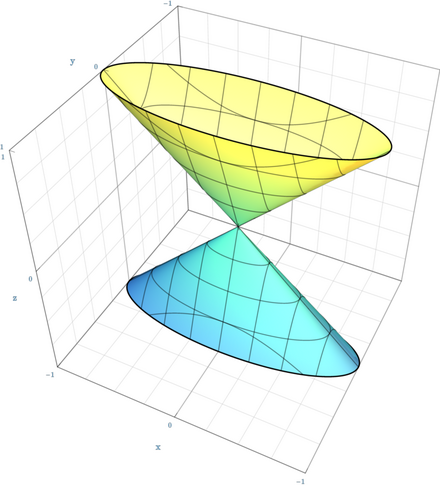
\includegraphics[width=0.4\linewidth]{divisor}
			\caption{$xy=z^2$}
			\label{fig:divisor}
		\end{figure}
		
		\item $X$=$\frac{\Spec\C[x,y,z,w]}{(xy-zw)}$. So $D=L=\{x=z=0\}$.
	\end{itemize}
\end{example}
\begin{defn}
	$D$ is \textbf{\textit{Q-Cartier}} if there exists $N$ such that $ND$ is Cartier.
\end{defn}
\begin{prop}[Regarding the last example]
	No multiple of $D_1$ is Cartier.
\end{prop}

\subsection{the hodge decomposition}
Now let's do some differential forms. Take local coordinates $z_1,\ldots,z_n$. We have that
\[df=f_1dz_1+\ldots+f_ndz_n\]
for
\[f_i=\frac{\partial}{\partial z_i}f_i:=\partial_if.\]
Now define
\[z_k=x_k+iy_k\qquad\text{and}\qquad\bar{z}_k=x_k-iy_k.\]
So $dx_1,dy_1,\ldots,dx_n,dy_n$ is a basis of $\Omega^{1,\Cinf}$. Now multiply by $\C$ to get $\overset{\Cinf}{T^*}\otimes_\R\C$ which is where the basis forms
\[dz_k=dx_k+idy_k\qquad\text{and}\qquad d\bar{z}_k=dx_k-idy_k\]
live. Also we have the map
\begin{align*}
	d:\Oc_X&\to\overset{\Cinf}{T^*}\otimes_\R\C\\
	f&\mapsto df
\end{align*}
And there exist some functions $G_{k\ell}(z,\bar{z})$ to change from some coordinates $z_k$ to other coordinates $w_k$.

Recall that
\begin{align*}
	\ell(\Lc)&=h^0(\Lc)=\dim\Gamma(X,\Lc)\\
	\ell(D)&=\ell(\Oc(D))\\
	h^k(E)&=\dim H^k(X,E).
\end{align*}
And then recall very quickly that for a vector space $V$ we have a \textbf{\textit{almost complex structure}} $J\in\End(V)$ such that $J^2=\id$ which has eigenvalues $\pm1$ (forcing the dimension of $V$ to be an even number) and complexify $V_\C:=V\otimes_\R\C$ to obtain the eigenspace decomposition
\[V^{1,0}_{\C}:=\ker(J-i)\qquad\text{and}\qquad V^{0,1}_{\C}:=\ker(J+i).\]
\begin{remark}
	A complex structure on a vector simulates the case of the operator $z\mapsto \sqrt{-1}z$ on the vector space of complex numbers. Recall that the operator $-\id$ on an euclidean space is orientation-preserving for even real-dimensions, such as those of the vector spaces $\C^n$. Thus, the operator $J$, which is interpreted as a rotation by 90 degrees, is composed with itself to yield an orientation-preserving isometry, $-\id$.
	
	In \href{https://en.wikipedia.org/wiki/Linear_complex_structure#Definition_and_properties}{wiki}, we see that A complex structure allows one to endow $V$ with the structure of a complex vector space. Complex scalar multiplication can be defined by
	\[(x+\sqrt{-1}y)v:=xv+yJ(v),\]
	and it is checked that this operation satisfies the axioms of a vector space over $\C$. {\color{cyan}Probably this is what we mean when we say we have \textbf{\textit{complexified}} the space $V$ to produce $V\otimes_\R\C$. The key of this reasoning is that this tensor product of two real vector spaces succesfully yields a complex vector thanks to $J$.}
	
	Futher in the same \href{https://en.wikipedia.org/wiki/Linear_complex_structure#Definition_and_properties}{wiki}, we find that it is not hard to see that every even-dimensional vector space admits a complex structure. One can define $J$ on pairs $e,f$ of basis vectors by $Je = f$ and $Jf = -e$ and then extend by linearity to all of $V$. If $(v_1, \ldots, v_n)$ is a basis for the complex vector space $V_J$, then $(v_1,Jv_1,\ldots,v_n,Jv_n)$ is a basis for the underlying real space $V$.
	
	Finally, A real linear transformation $A : V \to V$ is a \textbf{\textit{complex linear transformation}} of the corresponding complex space $V_J$ if and only if $A$ commutes with $J$, i.e. if and only if
	\[AJ=JA\]
	Likewise, a real subspace $U$ of $V$ is a \textbf{\textit{complex subspace}} of $V_J$ if and only if $J$ preserves $U$, i.e. if and only if
	\[JU=U.\]
\end{remark}
\begin{remark}
	Here's another interesting remark from \cite{piccione}, 1.4.24: Observe that if $(V,J)$ is a complex space endowed with a Hermitian product $g_s$, then the real part of $g_s$ is a positive inner product $g$ on $V$ and the imaginary part of $g_s$ is a symplectic form on $V$. 
\end{remark}

Back to our lecture, $J$ induces a map on the dual vector space
\[J:V\to V^*\]
given by
\[Jf(v)= f(Jv)\]
and in fact that goes all the way to
\[\mathbb{J}:\extp^{\bullet}V_{\C}^*\]
And then that Grassman algebra has a natural decomposition because each copy of $V^*_\C$ is already $V^*_{\C}=V^{0,1}\oplus V^{1,0}$ so we will denote equivalently by
\[\Ac^{p,q}=\extp^{p,q}T^*_{\C}=\Omega^{p,q}\]
\begin{remark}[\cite{voisin-intro}]
	The decomposition
	\begin{equation}\label{eq:hodge-decomposition1}
		T_{X,x}\otimes\C=T^{1,0}_{X,x}\oplus T^{0,1}_{X,x}
	\end{equation}
	induced by the almost complex structure $J_x$ that every tangent space of a complex manifold naturally induces a similar decomposition on the bundles of differential forms
	\[\Omega_{X,\C}^k:=\Omega_{X,\R}^k\otimes\C=\bigoplus_{p+q=k}\Omega_X^{p,q},\]
	where
	\begin{equation}\label{eq:hodge-decomposition2}
		\Omega^{p,q}_X\cong \extp^p\Omega^{1,0}_X\otimes\extp^q\Omega^{0,1}_X
	\end{equation}
	and
	\[\Omega_{X,\R}\otimes\C=\Omega^{1,0}_X\oplus\Omega^{0,1}_X\]
	is just the dual decomposition of \cref{eq:hodge-decomposition1}. The decomposition \cref{eq:hodge-decomposition2} has the property of Hodge symmetry
	\[\overline{\Omega_X^{p,q}}=\Omega^{q,p}_X,\]
	where complex conjugation acts naturally on $\Omega^k_{X,\C}$.
\end{remark}
Back to our lecture, we have de Rham differentials 
\begin{align*}
	\Ac^{0,0}&\overset{d}{\to}\Ac^{1,0}\oplus\Ac^{0,1}\\
	\Ac^{0,0}&\overset{\partial}{\to}\Ac^{1,0}\\
	\Ac^{0,0}&\overset{\bar\partial}{\to}\Ac^{0,1}
\end{align*}
so that $d=\partial+\bar\partial$. (Alternative notation is $d=d'+d''$.) And in general:
\begin{align*}
	\Ac^{p,q}&\overset{d}{\to}\Ac^{p+1,q}\oplus\Ac^{p,q+1}\\
	\Ac^{p,q}&\overset{\partial}{\to}\Ac^{p+1,q}\\
	\Ac^{p,q}&\overset{\bar\partial}{\to}\Ac^{p,q+1}
\end{align*}
and $J$ is \textbf{\textit{integrable}} if $\bar\partial^2=0$ which means that we not only have the de Rham complex but also its complex version $(\Ac^{p,\bullet},\bar\partial)$.
\begin{lemma}[$\partial\bar\partial$, Grothendieck $\sim$1958]
	$H^\bullet(\Ac^{p,\bullet},\bar\partial)=\Omega^p_X[0]$ there's an exact long sequence of sheaves
	\[\begin{tikzcd}
		\Omega_X^p\arrow[r]&\Ac^{p,0}\arrow[r,"\bar\partial"]&\Ac^{p+1}\arrow[r]&\cdots
	\end{tikzcd}\]
\end{lemma}
which means there is a resolution of holomorphic functions and we may compute cohomology. So we will know the \textbf{\textit{Hodge numbers}}
\[h^{p,q}(X):=h^q(\Omega^p_X).\]

Back to divsors,
\[\Gamma(U,\Oc(D))=\{f\in\Mc_X(U),(f)+D\geq0\}\]
and the divisor is
\[D=\underbrace{D_+}_{\text{zeroes}}-\underbrace{D_-}_{\text{poles}}\]
\paragraph{important results}
\begin{thm}[Riemann-Roch]
	\[\chi(X,\Lc):=\sum(-1)^kh^k(X,\Lc)\]
	\[\chi(X,\Lc)=\int_X\ch(\Lc)-Tdx\]
\end{thm}
\begin{thm}[Kodaira vanishing theorem]
	\[h^k(X,\omega_X(D)=0)\]
	for all $k>0$ if $D$ is ample.
\end{thm}
\begin{thm}[Serre duality]
	\[H^?(X,\Lc)^\vee=H^{n-k}(X,\omega_X\otimes\Lc^*)\]
\end{thm}
\begin{thm}[Hodge]
	For some subclass of $\Mfld$, Khäler,
	\[H^n(X,\C)=\bigoplus H^{p,q}.\]
\end{thm}
From \cite{voisin-intro}: the most important theorem proved in this book is the following:
\begin{thm}
	Let $H^{p,q}(X) \subset H^k(X,\C)$ be the set of classes which are representable by a closed form $\alpha$ which is of type $(p,q)$ at every point $x$ in the decomposition \cref{eq:hodge-decomposition2}. Then we have a decomposition
	\[H^k(X,\C)=\bigoplus_{p+q=k}H^{p,q}(X).\]
\end{thm}
Now consider the graded ring
\[R(X,\Lc)=\bigoplus_{k\geq0}\Gamma(X,\Lc^{\otimes k}).\]
It can be finitely generated or not. If $X$ is compact and $\Lc$-ample, however, yes. In fact
\[\kod(X,\Lc)=\]
\[\kod(X,\text{ample})=\dim X\]
\[\kod(X):=\kod(X,\omega_X)\]
and plurigenera are dimensions of the components of the graded ring $R(X,\Lc)$, that is,
\[\operatorname{pm}(X):=\dim\Gamma(X,\omega_X^{\otimes k})\]
and also
\[p_m(X)\sim m^{\kod(X)}\cdot c,\]
\[ae\in\{-\infty,0,1,2,\ldots,\dim X\}.\]
Where $-\infty$ stands for $p_m=0\;\forall m>0$.

Call $R(X,\omega_X)$ the \textbf{\textit{canonical ring}}.
\begin{thm}[Caseini, et al. 2006]
	$X$ compact, bipar
\end{thm}
Also define the \textbf{\textit{algebraic dimension}} to be
\[a(X)=\trdeg\Gamma(X,\Mc_X).\]
\begin{thm}[Siegel]
	If $X$ is compact,
	\[a(X)\leq\dim_\C X.\]
\end{thm}
And it turns out that $a(x)\geq\kod(X)$, and that $ae(X)\leq a(X)\leq \dim X$.
\subsection{three classical problems - 3apr}
\begin{question}[first Cousin problem, additive]
	In 1d Mittag-Leffler theorem.
	\[\Gamma(X,\Mc)\to\Gamma(X,\Mc/\Oc)\]
	is surjective? Injective?
	
	Suppose $X=\bigcup U_i$. Given $f_i\in\Gamma(U_1,\Mc)$ s.t. $f_i-f_j\in\Gamma(U_{ij},\Oc)$ does there exist $f\in\Gamma(X,\Mc)$ s.t. $f_i-f_j\in\Gamma(U_{j},\Oc)$?
	
	In this case we have
	\[\begin{tikzcd}
		\Gamma(X,\Mc)\arrow[r]&\Gamma(X,\Mc/\Oc)\arrow[r,"\delta"]&H^1(X,\Oc)
	\end{tikzcd}\]
\end{question}
\begin{question}[second Cousin problem, multiplicative]
	(In 1d-Weierstrass theorem)
	\[\Gamma(X,\Mc^*)\to\Gamma(X,\Mc^*/\Oc^*)\]
	
	Suppose $X=\bigcup U_i$. Given $f_i\in\Gamma(U_1,\Mc)$ s.t. $f_i/f_j\in\Gamma(U_{ij},\Oc)$ does there exist $f\in\Gamma(X,\Mc)$ s.t. $f_i/f_j\in\Gamma(U_{j},\Oc)$?
	
	Is it true that every Cartier divisor is a divisor of a {\color{cyan}holomorphic (?)} function?
	
	So Weierstrass theorem says for any discrete set in a disk there's a holomorphic function that vanishes in this discrete set. This is a generalization of that theorem.
	
	Now we have
	\[\begin{tikzcd}
		\Gamma(X,\Mc)\arrow[r]&\Gamma(X,\Mc/\Oc)\arrow[r,"\delta"]&H^1(X,\Oc^*)=\Pic(X)
	\end{tikzcd}\]
\end{question}
\begin{question}[Poincaré problem]
	Given $f\in\Gamma(X,\Mc)$ does there exists a pair $P,Q\in\Gamma(X,\Oc)$ such that
	\[f=\frac{P}{Q}\]
	and $P,Q$ are everywhere coprime? (for all $x\in X$, $P,Q\in\Oc_{X,x}$ are coprime?) 
\end{question}
\textbf{Today:}
\begin{claim}
	$H^1(X,\Oc)=0$ for polydisks and punctures polydisks.
\end{claim}
\begin{coro}
	$H^k(X,\Oc)=0$ for polydisks and punctures polydisks.
\end{coro}
\begin{lemma}
	For every divisor $D$ exists a unique decomposition $D=Z-P$ with $Z,P\geq0$, $\min(Z,P)>0$.
\end{lemma}
If $X$ is compact, then $f$ is determined $f\in\Mc_X^*$ by $f$ up to a constant.
\[(f)=(g)\iff\exists\lambda\in\C^*:f=\lambda g\]
\begin{claim}
	\[S^kV^*\to\Gamma(\P(V),\Oc(k))\]
	is surjective (which implies it is an isomorphism.)
\end{claim}
\begin{proof}
	Done in lecture, uses Hartog's theorem.
\end{proof}
\begin{remark}
	If $D\subset\P(V)$ is a hypersurface it is algebraic.
\end{remark}
Then let's do the hard work.
\begin{lemma}[Poincaré $\bar\partial$-lemma in 1 dimension]
	(Serre-58, from unpublished by Grothendieck and Polbeant. Find in \cite{griffiths} p 5, \cite{voisin-intro} ch 1, \cite{huybrechts} ch 1.)
	
	Let $\Omega$ be a domain in $\C$. For all $g\in\Cinf(\Omega,\C)$, for all point $p\in\Omega$ there exists a neighbourhood $U$ of $p$ and a function $f\in\Cinf$ such that
	\[\frac{\partial f}{\partial\bar{z}}g.\]
\end{lemma}
\begin{proof}
	Define \[g:=P(z)*_zf\sim\int \frac{f(w)}{z-w}dw\wedge d\bar w\]
	where $\sim$ means \textit{proportional} and $*$ is convolution.
\end{proof}
\begin{remark}
	If for all $i$ we have $\partial_{\bar u_i}f=0$ then $\partial_{\bar u_i}g$ for all $i$.
\end{remark}

\begin{lemma}[$\bar\partial$-Poincaré lemma for $q>0$]
	Given $\alpha\in\Ac^{p,q}(\bar B_r)$ such that $\bar\partial \alpha=0$ there exists $\varepsilon$ and  $\beta\in\Ac^{p,q-1}(\bar B_{r-\varepsilon})$ such that $\alpha=\bar\partial\beta$. That is, the \textbf{\textit{Dolbeaut complex}}
	\[\begin{tikzcd}
		\cdots\arrow[r]&\Ac^{p,q-1}\arrow[r,"\bar\partial"]&\Ac^{p,q}\arrow[r,"\bar\partial"]&\Ac^{p,q+1}\arrow[r]&\cdots
	\end{tikzcd}\]
	is \textit{locally} exact.
\end{lemma}
\begin{remark}\leavevmode
	\begin{itemize}
		\item The fact that $\bar\partial^2=0$, that is, that the Dolbeaut complex is a complex, is consequence of integrability.
		\item Also by computation, the cohomology of
		\[\begin{tikzcd}
			0\arrow[r]&\Ac^{p,0}(E)\arrow[r]&\Ac^{p,1}(E)\arrow[r]&\cdots
		\end{tikzcd}\]
		is $\Gamma(X,\Omega^p\otimes E)$, where $\Omega^p\otimes E$ are holomorphic sections.
	\end{itemize}
\end{remark}

\subsection{geometric structures}
\begin{defn}\leavevmode
	\begin{itemize}
		\item $I\in\End(V)$ such that $I^2=-\id$ is an \textbf{\textit{almost-complex structure}}
		\item $g$ symmetric bilinear form over $\R$.
		\item $\omega$ antisymmetric bilinear form over $\R$.
		\item $h$ hermitian form bilinear over $\R$ but anilinear over. It is \textbf{\textit{sesquilinear}}, that is, for $\alpha,\beta\in\C$,
		\[h(\alpha u,\beta v)=\bar\alpha\beta h(u,v).\]
		Also, if we define $\bar V$ as the vector space with the same vectors as $V$ but with the scalar product $\alpha * v=\bar\alpha v$, we have
		\begin{align*}
			\bar V\otimes V&\to\C
		\end{align*}
		So the definition of \textbf{\textit{Hermitian}} form is that $h(v,u)=\overline{h(u,v)}$.
	\end{itemize}
\end{defn}
Here are some relations. Given a Hermitian form $h$, we define $g=\Re h$ and $\omega=-\Im h$ to obtain
\begin{equation}\label{eq:2-3}
	h=g-i\omega.
\end{equation}
The point is that given $I$ and any one of $g,\omega$ or $h$ we can determine the remaining two. So for example start with $h$ hermitian, then \cref{eq:2-3} implies
\[\overline{h(v,u)}=\overline{g(v,u)-i\omega(v,u)}=g(v,u)+i\omega(v,u)\]
which implies that $g(u,v)=g(v,u)$ and $\omega(u,v)=-\omega(v,u)$.
So we have three sets of data:
\begin{enumerate}
	\item $(I,h)$
	\begin{itemize}
		\item $h$ hermitian which means two things: $h(v,u)=\overline{h(u,v)}$ and
		\item $h(-Iv,u)=h(u,Iv)=ih(u,v)$.
	\end{itemize}
	\item $(I,g)$
	\begin{itemize}
		\item $g(u,v)=g(v,u)$ and
		\item $g(Iu,Iv)=g(u,v)$.
	\end{itemize}
	\item $(I,\omega)$
	\begin{itemize}
		\item $\omega(u,v)=\omega(v,u)$
		\item $\omega(Iu,Iv)=\omega(u,v)$.
	\end{itemize}
\end{enumerate}
Also notice that \textbf{\textit{positivity}} means, $\forall u$,
\begin{itemize}
	\item For $g$, that $g(u,u)\geq0$ and $g(u,u)=0\iff u=0$.
	\item For $h$, that $h(u,u)\geq0$.
	\item For $\omega$, that $\omega(Iu,u)=\omega(u,-Iu)>0$.
\end{itemize}
And I think positivy in either of them implies positivity in the three. Use that $\omega(u,u)$ vanishes.

We also have the Lie groups
\[\O(2n,\R)=\O(V,g),\qquad\Sp(2n,\R)=\Sp(V,\omega)\quad\text{and}\quad\GL(n,\C)=\GL_\C(V,I),\]
which are all contained in $\GL(2n,\R)=\GL_\R(V)$ and in fact, the intersection of any two of them is
\[\U(V,h)\]
\begin{defn}
	A \textbf{\textit{Khäler manifold}} is $(M,J;g,\omega,h)$ where $(M,J)$ is an almost-complex manifold,
	\begin{itemize}
		\item $J$ is integrable, that is $J:TM\to TM$ with $J^2=-\Id$, and is induced canonically by an holomorphic atlas,
		\item $\omega$ is closed, that is, $d\omega=0$,
		\item $g$ is a metric.
	\end{itemize}
\end{defn}
\begin{thm}[Newlander-Nimberg]
	A necessary condition for $J$ to be integrable is that bracket of homolomorphic sections is holomorphic, that is $[T^{1,0},T^{1,0}]\subset T^{1,0}$. Hard theorem by Newlander-Nimberg is that this condition is sufficient. Also, Voisin proves this for real analytic $J$, that is that
\end{thm}
\begin{defn}
	\[\extp^{1,1}_\R=\{B\in\extp^{1,1}:\forall u,v\in V^{1,0},\;B(u,v)=0\}\]
\end{defn}
\begin{claim}
	$\omega\in\bigwedge^{1,1}_\R$.
\end{claim}
\begin{thm}[Weak Lefschetz]
	If $\omega$ is Khäler,
	\begin{align*}
		H^k(M,\R)&\to H^{2n-k}(M,\R)\\
		\alpha&\mapsto \alpha\wedge[\omega]^{\wedge n-k}
	\end{align*}
	is an isomorphism.
\end{thm}
\begin{coro}
	$H^k\underbrace{\to}_{\wedge\omega} H^{k+2}$. $k<n\implies$ mono and $k\geq n\implies$ epi. So we have the very strong properties on Betty numbers:
	\[b_0\leq b_2\leq b_4\leq \ldots\leq b_{\text{diam}/2}\]
	\[b_1\leq b_3\leq b_5\leq\ldots\leq b_{\text{diam}/2}\]
\end{coro}

In local coordinates $z_1,\ldots,z_n$, we know that
\[T^*_\C=\Ac^{1,0}\oplus\Ac^{0,1}\]
and $dz_1,\ldots, dz_n$ is a basis over $\Cinf$ for $\Ac^{1,0}$ and $d\bar z_1,\ldots d\bar z_n$ a basis for $\Ac^{0,1}$. The dual construction for the tangent bundle is $T^{1,0}$ with basis $\partial_{z_i}$ and $T^{0,1}$ with $\partial_{\bar{z}_i}$.

Next we have $\Ac^{1,1}=\Ac^{1,0}\otimes_\Cinf\Ac^{0,1}$ with basis $dz_i\otimes d\bar z_j$ which in fact is just the same as $dz_i\wedge d\bar z_j$ by linear algebra since there is an isomorphism
\[\extp^2(U\oplus V)=\extp^2U\oplus U\otimes V\oplus\extp^2U.\]
 Now fix
\[\omega=\sum_{i,j=1,\ldots, n}dz_i\wedge d\bar z_j,\]
where $\omega_{ij}\in\Cinf\otimes\C=\Ac^0$. We impose the \textbf{\textit{reality condition}} of $\omega=\bar\omega$, which is equivalent by a acomputation to $\omega_{ij}=-\bar\omega_{ji}$.

Then we compute
\[\omega(a^i\partial_i+b^j\partial_{\bar j})=\omega_{ij}(a^id^j-b^jc^i).\]
So fixing $a^i\partial_j:=u$ and $b^j\partial_{\bar j}:=v$ we get
\begin{align*}
	\omega(u+v,I(u+v))&=\omega_\C(u+v,\sqrt{-1}u-\sqrt{-1}v)\\
	&=\sqrt{-1}\omega(u+v,u-v)\\
	&=2\sqrt{-1}
\end{align*}
Now consider
\[\begin{tikzcd}
	&\Ac^{1,0}\arrow[dr,"-\bar\partial"]\\
	\Ac^{0,0}=\Cinf\arrow[rr,"i\partial\bar\partial"]\arrow[ur,"\partial"]\arrow[dr,"\bar\partial",swap]&&\Ac^{1,1}\\
	&\Ac^{0,1}\arrow[ur,"\partial",swap]
\end{tikzcd}\]
\begin{defn}
	A function $f\in\Ac^{0,0}$ is called \textbf{\textit{psh (pluri-subharmonic)}} if $\partial\bar\partial f$ is Kähler form.
\end{defn}
By simple computations we can show it is closed, real and of type $1,1$.
\begin{defn}
	 If locally on $U$ we have that $\omega=i\partial\bar\partial f$, then $g$ is called a local \textbf{\textit{Khäler potential}} for $\omega$.
\end{defn}
\begin{defn}[Alternative (official) definition of psh]
	$f:\Omega\to\R$ is psh if for any line we have
	\[f(u)\leq\int_{B(u,r)}f(z)\Vol_B=\int_{B(u,r)}f(z)\frac{dxdy}{\Area(B)}\]
\end{defn}
We have also defined \textbf{\textit{Hessian metrics}}, which are defined on coordinate systems in contrast to psh functions.
\begin{examples}[of psh functions]\leavevmode
	\begin{itemize}
		\item $f=\sum_k|z_k|$.
		\item $\log|z_i|^2$.
	\end{itemize}
\end{examples}
\begin{exercise}
	$\mathbb{P}^n$ is Kähler.
\end{exercise}
\subsection{homology class of a complex submanifold}

\begin{remark}[2.3.11, Huybrechts]
	Suppose $Y\subset X$ is a smooth hypersurface of a complex manifold $X$ of dimension $n$. In particular, $Y$ is a real codimension two submanifold of a compact manifold and thus defines an element $[Y]\in H^{2}(X,\mathbb{R})$, its \textit{\textbf{fundamental class}} as follows. By Poincar\'e duality, the linear map $\alpha\mapsto \int_{Y}\alpha)$ on $H^{2n-2}(X,\mathbb{R})$ defines an element on $H^{2}(X,\mathbb{R})$.
\end{remark}

Hodge conjecture asks which cohomology classes are submanifolds. Consider $X\hookrightarrow Y$ with $Y$ compact and $X$ closed submanifold (or subvariety).

\begin{enumerate}
	\item There is a class $[X]\in H^{2k}(Y,\R)$.
	\item $[X]\in H^{2k}(Y,\Z)$.
	\item $[X]\in H^{k,k}(Y,\C)$.
\end{enumerate}
Items 2. and 3. imply $[X]\in H^{k,k}(Y,\Z)\subset H^{k,k}(Y,\C)$.
\begin{conjecture}[Hodge]
	
	$\forall\alpha\in H^{k,k}(Y,\Q)\exists N$ and $X\hookrightarrow Y$ such that $N[X]=\alpha$.
\end{conjecture}
Which in fact implies \textbf{\textit{Grothendieck's standard conjectures}}.
\begin{thm}[Lefshetz theorem on $(1,1)$-classes]
	Hodge conjecture is true for $k=1$.
\end{thm}
\begin{thm}[Hard Lefshetz theorem]
	Hodge conjecture for $k$ implies Hodge conjecture for $\dim Y-k$.
\end{thm}
\subsection{fano manifolds}
\begin{defn}
	$X$ is \textbf{\textit{Fano manifold}} if $K_X$ is ample.
\end{defn}
\begin{thm}
	$\pi_1(X)=0$.
\end{thm}
\begin{proof}[Proof 1]
	KMM/Campion(?) Fano $\overset{\text{hard}}{\implies}$ rationally connected $\implies$ $\pi_1=0$.
\end{proof}
\begin{proof}[Proof]
	Fano implies exists Khäler metric $g$ such that $\Ric(g)>0$.
\end{proof}
\begin{thm}[Serre's homological criterion of ampleness]
	$\Lc\in\Pic(X)$ is ample if and only if for all $\Fc\in\Coh X\;\exists N$ such that $\forall n\geq N$ and $\forall k>0$,
	\[H^k(X,\Fc\otimes\Lc^{\otimes n})=0.\]
	It is equivalent that this condition holds for all $\Mc\in\Pic X$.
\end{thm}
\begin{thm}[Kleiman-Mori criterium for ampleness]
	$D$ is ample if for all $\beta$ in the Mori Cone of $X$ we have
	\[D\cdot\beta>0.\]
\end{thm}
\begin{defn}
	We define the \textbf{\textit{group of $k$-cycles}} as
	\[Z_k(X)=\bigoplus_{\substack{Y\subset X\\\text{irreducible}\\k\text{-dimensional}\\\text{complex}\\\text{subvarieties}}}\Z\cdot[Y]\]
\end{defn}
\begin{remark}
	On $Z_k(X)$ there are 4 equivalence relations:
	\begin{enumerate}
		\item Rational equivalence. For $k=n-1$ this is just linear equivalence of divisors.
		\item Algebraic equivalence.
		\item Homological equivalence.
		\item Numerical equivalence.
	\end{enumerate}
\end{remark}
\begin{defn}
	$Y\sim Y'\in Z_F(X)$ with $Y=\sum a_iY_i$ for $a_i\in\Z$, $Y'=\sum b_jYj$ with $b_j\in\Z$, if there exists
	\[Z\in Z_{k-1}(\P^1\times X)\]
	such that
	\[Z\cap X_0\in Z_k(X_0)=Z_k(X)\quad\text{and}\quad Z\cap X_\infty\in Z_k(X_\infty)=Z_k(X).\]
\end{defn}
\begin{exercise}
	Prove that rational equivalence of divisors is a linear equivalence.
\end{exercise}
\begin{defn}[Algebraic equivalence]
	Replace $\P^1$ by any connected algebraic variety or just by any smooth algebraic curve $C$. Then $Z\subset X\times C$ and for $P,Q\in C$,
	\[P_0=?\]
\end{defn}
[…]
\begin{defn}
	A divisor $D$ is called \textbf{\textit{numerically effective (nef)}} if for any curve $C\subset X$, $D\cdot C\geq0$.
\end{defn}
[…]
First recall that
\begin{thm}[Grauert]\leavevmode
	\begin{itemize}
		\item For all $k$, $h^k(E)<\infty$.
		\item $\#\{k:h^k(E)\neq0\}<\infty$
	\end{itemize}
\end{thm}
\begin{thm}[Hirzebruch-Riemann-Roch (HRR)]
	$E$ vector bundle (or, more generally, $\Fc\in\Coh(X)$), $X$ compact complex manifold (eg. projective).
	\[\chi(X,E)=\int_{[X]}\ch(E)\smile \Td_X\]
	where
	\begin{itemize}
		\item $\chi(X,E):=\sum(-1)^k\dim H^k(X,E)$.
		\item $\ch(E)$ is the \textbf{\textit{Chern character}}, that is, for $E=\Lc$,
		\[\ch(\Lc):=\exp(c_1(\Lc))\]
		for
		\[c_1(\Lc)=H=\underbrace{1}_{\in H^0}+\underbrace{H}_{\in H^2}+\underbrace{\frac{H^2}{2}}_{\in H^4}+\ldots\]
		so in general $\frac{H^k}{k!}\in H^{2k}(X,\Q)$ and
		\begin{align*}
			\ch(E\oplus F)&=\ch(E)+\ch(F)\\
			\ch(E\otimes F)&=\ch(E)\smile\ch(F)
		\end{align*}
		so there's a map
		\[\ch:\VectBund(X)\to K^{\top}(X)\to H^{2\bullet}(X,\Q)\]
		\item For $\Td_X$ define the \textbf{\textit{Todd function}}
		\[\td(x):=\frac{x}{1-e^x}=1+\frac{x}{2}+\frac{x}{12}+\ldots\]
		so its coefficients are Bernoulli numbers.
		
		Then for $\Lc\in\Pic(X)$ and $H=c_1(\Lc)$,
		\[\Td(\Lc):=\td(c_1(\Lc))=\td(H).\]
		And then
		\[\Td(E\oplus F)=\Td(E)\smile\Td(F)\]
		\begin{claim}
			There exists a unique map $\VectBund(X)\to H^{\bullet}(X,\Q)$ such that for the map
			\[Y\overset{f}{\to}E/X\]
			we have
			\[\Td(f^*z)=f^*\Td(E).\]
			Let us say that general characterstic classes (Chern classes)
			\begin{itemize}[label=$\circ$]
				\item $c(E)=\sum_{k=0}^\infty c_k(E)$
				\item $c_k(E)\in H^{2k}(X,\Z)$
				\item $c_0(E)=1$.
				\item $c(E\oplus F)=c(E)\smile c(F)$.
				\item $c(f^*E)=f^*c(E)$
			\end{itemize}
			and
			\begin{itemize}[label=$\circ$]
				\item $c(\Lc)=1+c_1(\Lc)$ as defined before.
			\end{itemize}
			Finally,
			\[\Td_X:=\Td(Tx)\]
			so
			\[\Td_X=1+\frac{c_1}{2}+\frac{c_1^2+c_2}{12}+\frac{c_1c_?}{24}+\ldots\]
		\end{claim}
	\end{itemize}
\end{thm}
\subsection{20 may}
There is a bilinear pairing
\[H_1(T,\Z)\times H_1(T,\Z)\to\Z\]
defined by intersection number.

\begin{thm}[Hodge Index (special case)]
	Suppose $\pi:X\to Y$ is a birrational map between a smooth projective surface $X$ and a projective surface $Y$. Then the signature of the intersection pairing betwen exceptional classes is negative definite.
\end{thm}
\begin{quotation}
	So we proved the Hodge index theorem for complex Khäler surfaces.
	
	All of this is end of third chapter in \cite{huybrechts}.
\end{quotation}
\subsection{22 may}
Recall
\begin{thm}[Hirzebruch-Riemann-Roch (HRR)]
	$E$ vector bundle (or, more generally, $\Fc\in\Coh(X)$), $X$ compact complex manifold (eg. projective).
	\[\chi(X,E)=\int_{[X]}\ch(E)\smile \Td_X\]
\end{thm}|
After long and hard computation, we have concluded that for a surface,
\begin{align*}
	\chi(X,\Lc)&=\Lc_X(1+c_1(\Lc)+\frac{1}{2}c_1^2(\Lc))\cdot\left(1+\frac{1}{2}c_1(X)+\frac{1}{12}(c_1^2(X)+c_2(X)\right)\\
	&=\int_X\frac{1}{12}(c_1^2(X)+c_2(X)+c_1(\Lc)\cdot\frac{1}{2}c_1(X)+\frac{1}{2}c_1^2(\Lc)
\end{align*}
We have derived Nöther formula:
\[\chi(X,\Oc_X)=\int_{[X]}\frac{c_1^2+c_2}{12}\]
Also there is the fact that
\[12\chi(X,\Oc_X)=K_X^2+e(X)\]
where $K$ is the \textbf{\textit{canonical degree}} and $e$ is the \textbf{\textit{Euler number}}.

Then we observed that $\chi(X,\Oc(D))$ is a quadratic form. Recall that
\begin{defn}
	If $A,B\in\Ab$, $f:A\to B$ is \textbf{\textit{quadratic}} if
	\[B(x,y)=f(x+y)-f(x)-f(y)-f(0)\]
	is bilinear.
\end{defn}
Define
\begin{align*}
	B(D_1,D_2)=&\chi(X,\Oc(D_1+D_2)-\chi(X,D_2)+\chi(X,\Oc_X))\\
	&=\frac{1}{2}(D_1^2+2D_1D_2+D_2^2)-D_1^2-D_2^2\\
	&D_1D_2
\end{align*}
It's also written in the board that
\[D_1D_2:=\chi(D_1+D_2)-\chi(D_1)-\chi(D_2)+\chi(\Oc)\]
\begin{claim}
	This function is symmetric and bilinear.
\end{claim}
\begin{proof}
	If $D_2$ is effective, $c\in (D_2)$. Consider
	\[\begin{tikzcd}
		0\arrow[r]&\Oc(-D_2)\arrow[r]&\Oc_X\arrow[r]&\Oc_C\arrow[r]&0
	\end{tikzcd}\]
	twist by $\Oc(D_1)$.
	\[\begin{tikzcd}
		0\arrow[r]&\Oc(-D_2D_2)\arrow[r]&\Oc(-D_1)\arrow[r]&\Oc_c(-D_1)\arrow[r]&0
	\end{tikzcd}\]
	So
	\[\chi(-D_1)=\chi(-D_2-D_1)+\chi(\Oc_c(-D_1))=\chi(C_1,\Oc(-D_1).\]
\end{proof}
Now we prove the Hodge index theorem
\begin{thm}
	Let $X$ be a projective surface. Let $H$ be very ample. Choose $0\neq D\in H^\perp$.
	\[D\cdot H=0\qquad\qquad \Pic(X)=ce(X)=H\oplus H^\perp.\]
	So we have an embedding $X\overset{|X|}{\hookrightarrow}\P^N$ and it turns out that
	\[H^2=\deg(X)>0.\]
	We will show that
	\[D^2<0.\]
\end{thm}
\begin{proof}
	\begin{claim}
		$D^2>0\implies DH\neq0\implies$ our theorem.
	\end{claim}
	\begin{proof}
		\[\chi(X,nD)\sim \frac{n^2D^2}{2}\quad\text{ for }n\gg 0\]
		and also
		\[\chi(X,nD)=h^0(nD)h^1(nD)+h^2(K-nD)=h^2(nD)\overset{n\to\infty}{\longrightarrow}\infty.\]
		Either
		\begin{enumerate}
			\item $h^0(nD)\to\infty$ as $n\to\infty$. This implies $DH>0$.
			\item $h^(K-nD)\to\infty$ as $n\to\infty$. This is implies $DH<0$.
			\begin{proof}[Proof of 1.]
				$nD$ is effective and $H$ is very ample, so $hDH>0\implies DH>0$.
			\end{proof}
			\begin{proof}[Proof of 2.]
				content...
			\end{proof}
		\end{enumerate}
	\end{proof}
\end{proof}
\subsection{blow-ups}
(Look in \cite{hartshorne}) Consider $Z\overset{i}{\hookrightarrow}X$ for $Z,X$ complex manifolds (for simplicity, more generally take analytic subspaces). Now consider
\[\begin{tikzcd}
	0\arrow[r]&\If_Z\arrow[r,hook]&\Oc_X\arrow[r]&\Oc_Z\arrow[r]&0
\end{tikzcd}\]
where $\If_Z$ is the \textbf{\textit{ideal sheaf}}, whose sections are
\[\Gamma(U,\If_Z)=\{f\in\Gamma(U,\Oc_X):f|_Z=0\},\]
and $\Oc_Z$ is the \textbf{\textit{quotient sheaf}} $\Oc_X/\If_Z$.

Notice $\supp(\Oc_Z)=Z$ where, in general the \textbf{\textit{support of a sheaf $\Fc$}} is $\supp\Fc=\{x\in X:\Fc\neq0\}$. \textbf{Important:} the support of a coherent sheaf is closed.

\begin{defn}
	\[\Bl_{\If}X=\Proj\bigoplus_{d\geq0}\If^d\]
	where $\Proj$ is defined as follows.
\end{defn}
\begin{defn}[1]
	Given a finitely generated sheaf of graded algebras $\Ac^\bullet=\bigoplus\Ac^d$ over $X$. This produces a triple
	\begin{itemize}
		\item A space $Y=\Proj_X\Ac$.
		\item A morphism $Y\to X$.
		\item Coherent sheaves $\Oc_Y(d)$ such that $\bigoplus_d\Oc_Y(d)$.
	\end{itemize}
	If $\Ac$ is generated over $\Oc_X$ in degree 1, then $\Oc_Y(d)$ are l.b. and $\Oc_Y(d)\aleph\Oc_Y(1)^{\otimes d}$ and $\Oc_Y(1)$ is relatively very ample.
	
	$f:Y\to X$ is \textbf{\textit{projective}} if there exists a closed embedding $j:Y\hookrightarrow Z$ and
	\[\begin{tikzcd}
		&X\times\P^N\arrow[dd,"\pi_1"]\\
		Y\arrow[ur,hook,"j"]\arrow[dr,"f"]&\\
		&X\arrow[r,hook]&Z\times \P^n\arrow[d]\\
		&&Z
	\end{tikzcd}\]
\end{defn}
\begin{defn}[2]
	An "alternative" ("more general") definition would be
	\[\begin{tikzcd}
		Y\arrow[r,hook,"j"]&Z\arrow[r,"\cong"]&\P_X(E)\arrow[r,"\pi_2"]&X
	\end{tikzcd}\]
	for a closed embedding $j$.
\end{defn}
However,
\begin{exercise}\leavevmode
	\begin{enumerate}
		\item Prove that definition 2 can be reduced to definition 1.
		\item Prove that composition of proj is proj.
	\end{enumerate}
\end{exercise}
\begin{remark}
	$\Proj$ is a modification of $\Spec$. The only new feature of $\Proj$ is that $\Ac$ is now \textit{graded}. (So ideals go to graded ideals, modules go to grades modules, etc…)
\end{remark}
The system of generators are going to be homogeneous coordinates on the $\Proj$.
\begin{example}[Twisted cubic]
	The twisted cubic is not a complete intersection. $\PGL(\U)$ acts everywhere.
\end{example}
\subsection{universal property of blow ups}
Let
\[\begin{tikzcd}
	Z\arrow[r,hook,"i"]&X&\Bl_ZX\arrow[l,"\pi"]
\end{tikzcd}\]
\begin{enumerate}
	\item $\Bl_2X\overset{\pi}{\to}X$ is a projective morphism.
	\item[1'.] $\pi$ is proper, ($1.\implies1'$)
	'item $\pi:\pi^{-1}(U)\to U$ is an isomorphism.
	\item $E=\pi^{-1}(Z)$, the \textbf{\textit{exact locus}}, is a Cartier divisor.
\end{enumerate}
\begin{prop}[Universal property of blow up]
	Blow up is a universal morphism with $1+3$ or $1'+3$. It means that
	\[\begin{tikzcd}
		E\arrow[r,hook]\arrow[d]&\Bl_ZX\arrow[d]&Y\supset D\arrow[l,dashed,swap,"\exists"]\arrow[dl,"f"]\\
		Z\arrow[r,hook]&X
	\end{tikzcd}\]
	So $f$ factors through the blow up.
\end{prop}

\subsection{lefschetz theorem about $(1,1)$-classes}
\begin{thm}[Lefschetz theorem about $(1,1)$-classes]
	If $X$ is a compact Kähler manifold, then any class in $H^{1,1}(X,\Z)$ is algebraic, that is, $c_1:\Pic X\to H^{1,1}(X,\Z)$ is surjective.
\end{thm}
\begin{proof}
	Consider
	\[\begin{tikzcd}
		0\arrow[r]&\Z\arrow[r,"i"]&\Oc\arrow[r]&\Oc^*\arrow[r]&0
	\end{tikzcd}\]
	and then
	\[\begin{tikzcd}
		H^2(X,\Z)\arrow[r,"\eta"]\arrow[d]&H^2(X,\Oc)=H^{0,2}(X)\\
		H^2(X,\Z)\otimes\C=H^2(X,\C)\arrow[r,equal]&H^{0,2}(X)\oplus H^{1,1}(X)\oplus H^{2,0}(X)\arrow[u,"\pi^{0,2}",swap]
	\end{tikzcd}\]
	We want to see that these two natural maps from $H^2(X,\Z)$ to $H^2(X,\Oc)$ are the same;
	\begin{enumerate}
		\item $\eta=H^2(Z\overset{i}{\hookrightarrow}\Oc)$ from long exact sequence of cohomology, and
		\item Hodge theory projection from $H^2(X,\C)\to H^{0,2}(X)$.
	\end{enumerate}
\end{proof}
\begin{exercise}
	Torsion in $H^2(X,\Z)$ is dual to torsion in $H_1(X,\Z)$.
\end{exercise}
\begin{remark}
	Next time we shall introduce \textbf{\textit{Hodge filtration $F^p\Ac^\bullet$}} and study various cohomologies associated to it
\end{remark}
\subsection{3 june}
We start by noticing that there is a morphism of complexes $j$ given by
\[\begin{tikzcd}
	\Ac^{k}\arrow[r,"d"]\arrow[d,"\pi^{0,k}",swap]&\Ac^{k+1}\arrow[d,"\pi^{0,k+1}"]\\
	\Ac^{0,k}\arrow[r,"\bar\partial"]&\Ac^{0,k+1}
\end{tikzcd}\]
(while the same is not true if we consider the complex $\Ac^{1,k}\to\Ac^{1,k+1}$ below.) This in turn induces cohomology maps $H^k(j):H^k(X,\C_X)\to H^k(X,\O_X)$ by diagram chasing. This holds for all complex manifolds. Then $\eta$ from last lecture is taken to be $H^2(j)$

Now we'll try to use Kählerness. Let $X$ be compact Kähler and so that for all $[\alpha]\in H^2(X,\C)$ exists $\tilde\alpha$ harmonic, ie. $d\tilde\alpha$, such that $[\tilde\alpha]=[\alpha]$. Then we have that $\eta_j[\alpha]=\eta_j[\tilde\alpha]=[\tilde\alpha^{0,2}]$.

By Hodge theory in compact Kähler, we have that $H_\partial^{2,0}(X)$ and $H^{2,0}_{\bar\partial}(X)$. Then we have that if $(\alpha,\beta)=0$, then for all $\beta\in\Ac^{2,0}\oplus\Ac^{0,2}$ closed, $\alpha\in\ker\pi^{0,2}\cap\ker\pi^{2,0}$, then $\alpha\in H^{1,1}_{\bar\partial}(X)$.

This proves Lefschetz $(1,1)$.

\begin{coro}
	If $X$ is a smooth complex projective variety, then for any $\alpha\in H^{2k}(X,\C)$ there exists $Y_i\subset X$ of codimension $k$ and $c_i\in\C$ such that
	\[\alpha=\sum c_i[Y_i].\]
\end{coro}
\begin{proof}
	Let's prove this corollary for $k=1$, that is, for the case of divisors. Consider tensor product by $\Q$ to obtain
	\[\Q\otimes\Div X\to H^2(X,\C)\]
	We also have the inclusion-induced
	\[H^{2k}(X,\Q)\to H^{2k}(X,\C)=\bigoplus_{p=q}H^{p,q}(X,\Q)\]
\end{proof}

\begin{remark}[Sergey, July 18 24']\leavevmode
	{\color{lavendermagenta}
		Lefschetz (1,1) theorem is the almost only known proven case of Hodge conjecture. And Daniel apparently misinterpreted it (and maybe mixed with more general conjecture, because his $k$ is arbitrary, not $k=1$).

		I think there are 2 right statements, that being mixed make a wrong statement.
		
		One is purely topological and unrelated to complex manifolds---any cohomology class on a smooth compact manifold is represent by a submanifold.

		Another is essentially the trivial part of Hodge conjecture. (Or non-trivial part of Lefschetz $(1,1)$.)

		One correct statement is purely topological:
\begin{enumerate}
		\item With a smooth compact manifold $M$ of real dimension $k$ {\color{persimmon}($n$?)} one can associate its fundamental class $[M]$ in $H_n(M,\mathbb{Z})$, and moreover it is a generator (we won't need the latter fact).

		{\color{persimmon}Recall here from Hatcher:
		\begin{thm}[3.26]\leavevmode
			Let $M$ be a closed connected $n$-manifold. Then
			\begin{enumerate}
				\item If $M$ is $\mathbb{R}$-orientable, the map $H_{n}(M;R)\to H_{n}(M,M-\{x\};R):=H_{n}(M|x;R)\cong R$ is an isomorphism for all $x\in M$.
				\item If $M$ is not $\mathbb{R}$-orientable, the map $H_{n}(M;R)\to H_{n}(M|x;R)\cong R$ is injective with image $\{r\in R:2r=0\} $ for all $x\in M$.
				\item $H_{i}(M;M)=0$ for $i>n$.
			\end{enumerate}
		\end{thm}
	An element of $H_{n}(M;R)$ whose image in $H_{n}(M|x;R)$ is a generator for all $x$ is called a \textit{\textbf{fundamental class}} for $M$ with coefficients in $R$.}

	\item Homology is covariant, so with $f : X \to Y$ there is $f_*$ or $H_k(f) : H_k(X) \to  H_k(Y)$
	\item So if $M$ is a compact smooth manifold of dimension $k$ and $Y$ is any space and $f:M\to Y$ is a continuous map, then there is an associated $f_{*}:H_{k}(M,\mathbb{Z})\to H_{k}(Y,\mathbb{Z})$, and an element $[M]\in H_{k}(M,\mathbb{Z})$, so \textit{\textbf{taking}}  $H_{k}(f)[M]$ we obtain some homology class in $H_{k}(Y,Z)$ which we can denote $[M,f]$ or by abuse of notation as $[M]$. Here one has to remember how $M$ is embedded (or mapped) intro $Y$.

	This gives a source of homology classes on $Y$. One may ask how special are the classes obtained this way.
	\end{enumerate}
	
	One question is topological:

	\begin{question}[Topological]
		When $Y$ is a smooth compact manifold, what subgroup of $H_{k}(Y,Z)$ is generated by classes $[M,f]$? What elements of $H_{k}(Y,Z)$ are representable as $[M,f]$?
	\end{question}

	Another is dif and only if erent, and belongs to complex (algebraic) geometry:

	\begin{question}[Complex-algebro-geometrical]
		If $Y$ is also a complex manifold (e.g. a smooth projective complex variety), what subgroup is generated by classes $[X,f]$ where $X$ is complex and $f$ holomorphic?
	\end{question}

	First question (topological) has positive answer, that basically says everything is realizable.

	Second question is essentially answered:
	\begin{itemize}
		\item For $H^{2}(Y,\mathbb{Z})$ and for $H_{2n-2}(Y,\mathbb{Z})$ by Lefschetz theorem on $(1,1)$-classes (and Poincar\'e duality) {\color{persimmon}(saying every class is algebraic)},
		\item for $H_{2}(Y,\mathbb{Q})$ (with rational coefficients) it is answered by the exam problem (the one with delivery date due to July 8).
	\item For $H_{2k}(Y,\mathbb{Q})$ where $1<k<n-1$ the conjectural answer is the Hodge conjecture.}
	\end{itemize}
\end{remark}



\begin{exercise}[Exam problem due June 8]
	Let $V$ be a smooth projective complex algebraic variety of dimension $n$. Prove that any homology class $C\in H_{2}(V,\mathbb{Q})$ the gollowing two conditions are equivalent:
	\begin{enumerate}
		\item \[\int_{C}\alpha=0\qquad \text{for all holomorphic 2-forms $\alpha$} \]
		\item There are algebraic curves  $X_{1},\ldots,X_{n}$ on $V$ and rational numbers $m_{1},\ldots,m_{n}$ such that
			\[C=m_{1}[X_{1}]+\ldots+m_{n}[X_{n}],\]
			here $[X_{k}]$ are homology classes of curves $[X_{k}]$ in $H_{2}(V,\mathbb{Q})$.
	\end{enumerate}
	\textbf{Bonus:} for which dimensions ($n=1,2,3,4,\ldots$) can you improve your proofs to replace $Q$ by $\mathbb{Z}$?
\end{exercise}

\begin{proof}[Solution]
	
\end{proof}

\subsection{$K$-group}
We have to categories: $\VectBund(X)$ and $\Coh(X)$. And two groups $K(X)$ and $G(X)$. Also there's $K^0(X)$ and $K_0(X)$. $K$-theory usually studied the case when we replace the $0$ with other numbers, but we won't do this, so we just use the notation without the $0$.

So, vector bundles form a ring with tensor product so we have $K(X)\to \Ring$. Now notice that $K_0(X)$ is a module over $K^0(X)$.

If $X$ is smooth and projective, by Serre, any coherent sheaf has a finite resolution by vector bundles. (If the variety is not smooth the resolution can become infinite.)

Now: $\supp(\Fc)\subset$ a closed algebraic subvariety. Consider a filtration, \textbf{\textit{topological filtration}} $G(X)$ and then $F^kG(X)$, the subgroup generated by sheaves $\Fc$. ``Filtration defined in terms of codimension of support". This leads to something like $K^0_{\alg}\to K^0_{\top}(X)$, which in turn reminds us to the Chow map.

What do we know about this topological filtration? Consider the Chow group $\CH^k(X)$ and $F^k(X)/F^{k+1}(X)$ and then there is the \textbf{\textit{associated graded}} $\Gr^k_FK(X)$. And then we may take direct sum over $k$ up to $\dim X$. And then how can we relate them?

For $k=0$ we have $\Z[X]$. On the other side $\Gr^0_FK(X)\to \Z$ we may take a section (an arrow going the other way).

For $k=1$ we have , and on the right side 
\begin{align*}
	\Gr^1_FK(X)&\to\Cl X\\
	\sum F_i&\mapsto\sum_ik(F_i)\cdot D_i
\end{align*}
Is this map surjective? Yesbecause $\sum a_i\Oc_{D_i}\mapsto\sum a_iD_i$. Is it injective? Yes yes, in principle yes.
\begin{claim}[Fulton, Intersection theory]
	There are two maps,
	\begin{align*}
		\begin{aligned}
			c:\Gr^k_FK(X)&\to\CH^k(X)\\
			E&\mapsto c_k(E)
		\end{aligned}\qquad\qquad
		\begin{aligned}
			\varphi:\CH^k(X)&\to\Gr_F^k(X)\\
			Z&\mapsto[\Oc_Z]
		\end{aligned}
	\end{align*}
	The first one is of course the $k$-th Chern class. So the claim is that they are \textit{almost} inverse of each other:
	\begin{align*}
		\varphi\circ c&=(-1)^k(k+1)!1_{\Gr^k_FK(X)}\\
		c\circ\varphi&=(-1)^k(k-1)!1_{\CH^k(X)}
	\end{align*}
\end{claim}

\subsection{weak lefshetz theorem, 5 june}
There is a \textbf{\textit{box product}} $E\boxtimes F=p_X^*E\otimes p_Y^*F$ for $E/X$ and $F/Y$ and
\[\begin{tikzcd}
	&X\times Y\arrow[dl]\arrow[dr]\\
	X&&Y
\end{tikzcd}\]
\begin{thm}[K\"unneth formula for cohomology of coherent sheaves]
	Let them be line bundles
	\[\Gamma(X\times Y,E\boxtimes F)=\Gamma(X,E)\otimes\Gamma(Y,F)\]
\end{thm}
\begin{thm}[semi-continuity]
	The function $w\to h^0(Z_W,\Fc|_{Z_W})$ is upper semi continuous on $W$.
	
	These are closed:
	\[W_k=\{w\in W:h(Z_W,\Fc_U)\geq k\}\]
	
	And also we can put an $r$ like this: $w\to h^r(Z_W,\Fc|_{Z_W})$ and this
		\[W_k=\{w\in W:h^r(Z_W,\Fc_U)\geq k\}\]
\end{thm}
\begin{example}[Abel's map]
	$S^k(X)\to\Pic^k(X)$.
\end{example}
\begin{thm}[Riemann]
	$\Theta\subset\Pic^{g-1}X$ already "knows" all other strata.
	\[\Mult_{\Lc}(\Theta)=h^0(X,\Lc)\]
\end{thm}
We also talked about
\begin{defn}
	An \textbf{\textit{incidence variety}} is when its elements are pairs of incident objects. So for example
	\[Z(\ev)=\left\{\sum X_iY_i=0\right\}\subset\P(V)\times\P(V^*)\]
	is an incidence variety. (It comes from considering the projectivizations of a vector space $V$ and its dual.)
\end{defn}
For $X\subset \P^N$ we may take a hyperplane $H\subset\P^N$. Notice that $H\cong\P^{N-1}$ and also it can be thought as an element of $\P^{N*}$. Define the \textbf{\textit{hyperplane section}} $X_H=X\cap H$.

Let $H\in\P(V^*)$ be a hyperplane such that $X_H$ is smooth. Lefshetz hyperplane theorem relates topology of projective variety $X$ and $X_H$.

\begin{thm}[Bertini]\leavevmode
	\begin{enumerate}
		\item There exists $H$ such that $X_H$ is smooth.
		\item It is Zariski-open (and dense).
	\end{enumerate}
\end{thm}
More generally, let $|H|$ be a linear system on a variety $X$ (with $\operatorname{char} k=0$). Let $\Lc\in\Pic X$. There's a map
\begin{align*}
	content...
\end{align*}
On the Telegram chat we have:
\begin{thm}[Bertini]
	Let $X\subset\P^n$ be a smooth variety. Then for a generic hyperplane $H$, the \textbf{\textit{hyperplane section}} $X_H=X\cap H$ is smooth.
	
	Equivalent formulation: projective dual of a smooth projective variety is no the whole $\P^{N*}$ but its proper subvariety.
\end{thm}

\begin{defn}\leavevmode
	\begin{enumerate}
		\item A \textbf{\textit{fixed divisor}} $D\subset X$ is an irreducible Weil dividor that is fixed if $\forall i$, $(s_i)\supset D$.
	
		\item The \textbf{\textit{fixed part of $|H|$}} is  $\bigcup$(fixed irreducible divisors).
		
		\item L.S. is \textbf{\textit{movable}} if $\Fix(|H|)=\varnothing$.
		
		\item \textbf{\textit{Base locus}} is the points where the point is not well-defined, ie. where it vanishes. So its \[B_S|H|=\{[V]:S_V=0\}=\{x\in X:s_i(x)=0\}\]
		it is a closed subvariety.
		
		\item More generally, let $|H|$ be a movable linear system on a variety $X$. The \textbf{\textit{singular locus}} $\Sing X$ …
	\end{enumerate}
\end{defn}
\begin{thm}[Also Bertini's]
	Then for generic $H\in|H|$, $\Sing H\subset\Sing X\cap B_S|H|$.
\end{thm}
For most varieties their projective dual is a hypersurface.
\begin{thm}[Lefshetz]
	For example, you can consider the maps
	\begin{align*}
		H^k(X,\Z)&\to H^k(X_H,\Z)\\
		H_k(X_H,\Z)&\to H_k(X,\Z)\\
		\pi_k(X_H)&\to\pi_k(X)
	\end{align*}
	Then
	\begin{enumerate}
		\item All these maps are isomorphisms for $k<\dim_{\R}X_H$. {\color{magenta}(Homework: This for $H^k$ is derivable from Hard Lefshetz theorem)}
		\item $H^k(i)$ is injective for $k=\dim X_H$, $H^k(i)$ is sujective and $\pi_k(i)$ is surjective.
	\end{enumerate}
\end{thm}



\begin{coro}
	$h^{p,q}(X_H)=h^{p,q}(X)$ for $p+q<\dim X-1$ and $h^{p,q}(X_H)\geq h^{p,q}(X)$ for $p+q=\dim_{\C}X-1$
\end{coro}
Do you know some statement that implies all of this? Some people prefer this form
\begin{thm}[Another variation]
	$(X\backslash X_H)$ is homotopy equivalent to CW complex $Z$ with cells of dimension less or equal to $\dim_{\C}X$, where $X\hookrightarrow\C$ is an affine variety.
\end{thm}
From standard algebraic topology that statement implies all of the others.
\begin{proof}[Idea of proof]
	We want to contract things. Construct some function on $X\backslash X_H$ whose critical locus is of dimension $\dim_{\C}X$. Now 
	\[x\mapsto\dist(x,X_H)^2\]
	is a smooth function and equals to zero on the complement of $X_H$. So consider points that are maximally far away.
\end{proof}
\begin{coro}
	If you have some hypersurface its Hodge numbers will be one, one, one and then all of this part even, at least one, this is non-primitive class, of course, mirror symmetry will rotate this for Calabi-Yau, which is unusual, it's strange, mirror of hypersurfaces is not hypersurface, big number here corresponds to big Picard number. You need to do some blow ups. \textbf{\textit{Complete intersection of Calabi-Yau (CISY)}}. Bundle is ample if all these numbers are positive. Can I remove the projective space? Can I make it not very ample line bundle, ample line bundle, there are some extensions of this theorem. Clear?
\end{coro}
Hori and Tong: Physical understanding of these hypersurfaces. It's related to mirror symmetry but not mirror symmetry. Related to this, the geometry, Fukaya categories. They have the same branes. Mirror symmetry is A-branes here, B-branes there. What space transition is doing.

\begin{exercise}
	Prove that
	\[H^k(X,\Z)&\to H^k(X_H,\Z)\]
	using hard Lefschetz theorem.
\end{exercise}

\begin{proof}[Solution]
	Based on \href{https://math.stackexchange.com/questions/712791/application-of-lefschetz-duality-to-prove-lefschetz-hyperplane-theorem}{StackExchange} and \href{https://en.wikipedia.org/wiki/Lefschetz_hyperplane_theorem}{wiki}. Also the proof is based on \cite{milnor}, coro. 7.3, it goes like this:

	The isomorphism $H^{k}(X,\Z)\cong H^{k}(X_H,\Z)$ is equivalent to the vanishing of the relative cohomology groups $ H^{k}(X,X_H,\Z)$ vanshing by the long exact sequence of the pair.

	To show this we need to adapt our hard LEfschetz to some relativ version. Milnor calls this \textit{\textbf{Lefschetz duality}}. The answer quoted above on StackEchange then refers to \cite{bredon}, chp VI thm 8.3, which states that
\begin{equation*}
	H^{k}(K,L;G)\cong H_{n-k}(M-L,M_-K;G)
\end{equation*}
for compact $L\subset K\subset M$, where the isomorphism is given by cap product in \v Cech cohomology.

Smartly choose $M=X$, $K=X-X_H$ and $L=\varnothing$ to get that $M-K$ is $X-(X-X_H)=X_H$. Then,
\begin{equation*}
	H_{n-k}(X,X_H;\Z)\cong H^{k}(X-X_H;\Z)
\end{equation*}
Finally Milnor says that since $X-X_H$ is a nonsingular algebraic variety in $\C^n$, it will have homotopy type of a CW complex (this is thm 7.2 in \cite{milnor}, and actually the last version of Lefschetz that we stated), and thus its cohomology will vanish. Let's try to understand what's going on here.

The statement we're looking for is \href{https://en.wikipedia.org/wiki/Andreotti–Frankel_theorem}{Andreotti-Frankel theorem}:

\begin{thm}[Andreotti-Frankel]
	If $V$ is a smooth, complex affine variety of complex dimension $n$ or, more generally, if $V$ is any Stein manofld of dimension $n$, then $V$ admits a Morse function with critical points of index at most $n$, and so $V$ is homotopy equivalent to a CW complex of real dimension at most $n$. 
\end{thm}

Consequently, if $V\subset \C^{r}$ is a complex manifold of dimension $n$ then $V$ has the homotopy thype of a CW complex of real dimension $\le n$. Therefore
\begin{equation*}
	H^{i}(V,\Z)=0,\qquad \text{for }i>0
\end{equation*}
and
\begin{equation*}
	H_{i}(V,\Z)=0,\qquad\text{for }i>0.
\end{equation*}
This theorem applies in particular to any smooth, complex affine variety of dimension $n$.

So, this makes the homology groups above $n$ vanish, but wanted them to vanish for $k<n$… anyway, Milnor actually states Lefschetz duality in a more convenient way:
\begin{equation*}
	H^{2n-k}(X_H;\Z)\cong H_{k}(X,X_H;\Z)
\end{equation*}
And then it makes more sense.

Is there another way of doing this other than by the CW-complex argument?
\end{proof}


\begin{question}[]
	How to prove Lefschetz hyperplane theorem?
\end{question}
\begin{proof}[Answer]
	The original proof of Lefschetz of his hyperplane section theorem used \textit{\textbf{Lefschetz pencils}}. This is a complex counter-part of a notion of a Morse function, and still popular today, e.g. Aroux, Donaldson, Katzarkov and co constructed and applied Lefschetz pencils for problems on symplectic geometry (they generalized notion of Lefschetz pencil to symplectic varieties).

	In projective algebraic geometry, a pencil of hyperplane sections of a smooth projective variety $X$ in $P$ is known as a \href{https://en.wikipedia.org/wiki/Lefschetz_pencil}{Lefschetz pencil} if any of its elements is either smooth or has a unique singular point, which is a Morse point (also known as ordinary double point).

	Bertini theorem in a form that we proved implies the existence of Lefschetz pencils: namely if $X\subset \P:=\P(V)$ is a smooth projective variety, and $X^*$ is its dual in $\P^*:=\P(V^*)$, then \textit{pencils of hyperplane sections are in bijection with projective lines $L$ in $\P^*$}. {\color{cyan}So, for example, sometimes lines are in correspondence with points:}
	\begin{figure}[H]
		\centering
		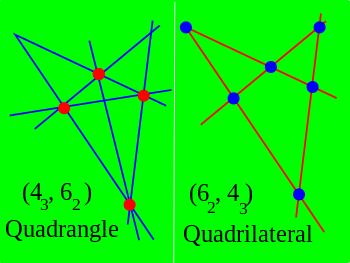
\includegraphics[width=0.4\textwidth]{duality}
	\end{figure}	
	A pencil is a Lefschetz pencil if the respective line $L$ intersects $X^*$ transversally. {\color{azure}This might be not immediately obvious, but follows after some analysis of local situation---exercise!} {\color{magenta}So I guess here a good question is what is $X^*$…} 

	If $\codim X^*>1$ (then variety $X$ is called \textit{\textbf{defective}} then there are some lines that do not intersect $X^*$ at all--- this means all elements in such pencil are smooth. This is quite rare (as we discussed).
	\begin{figure}[H]
		\centering
		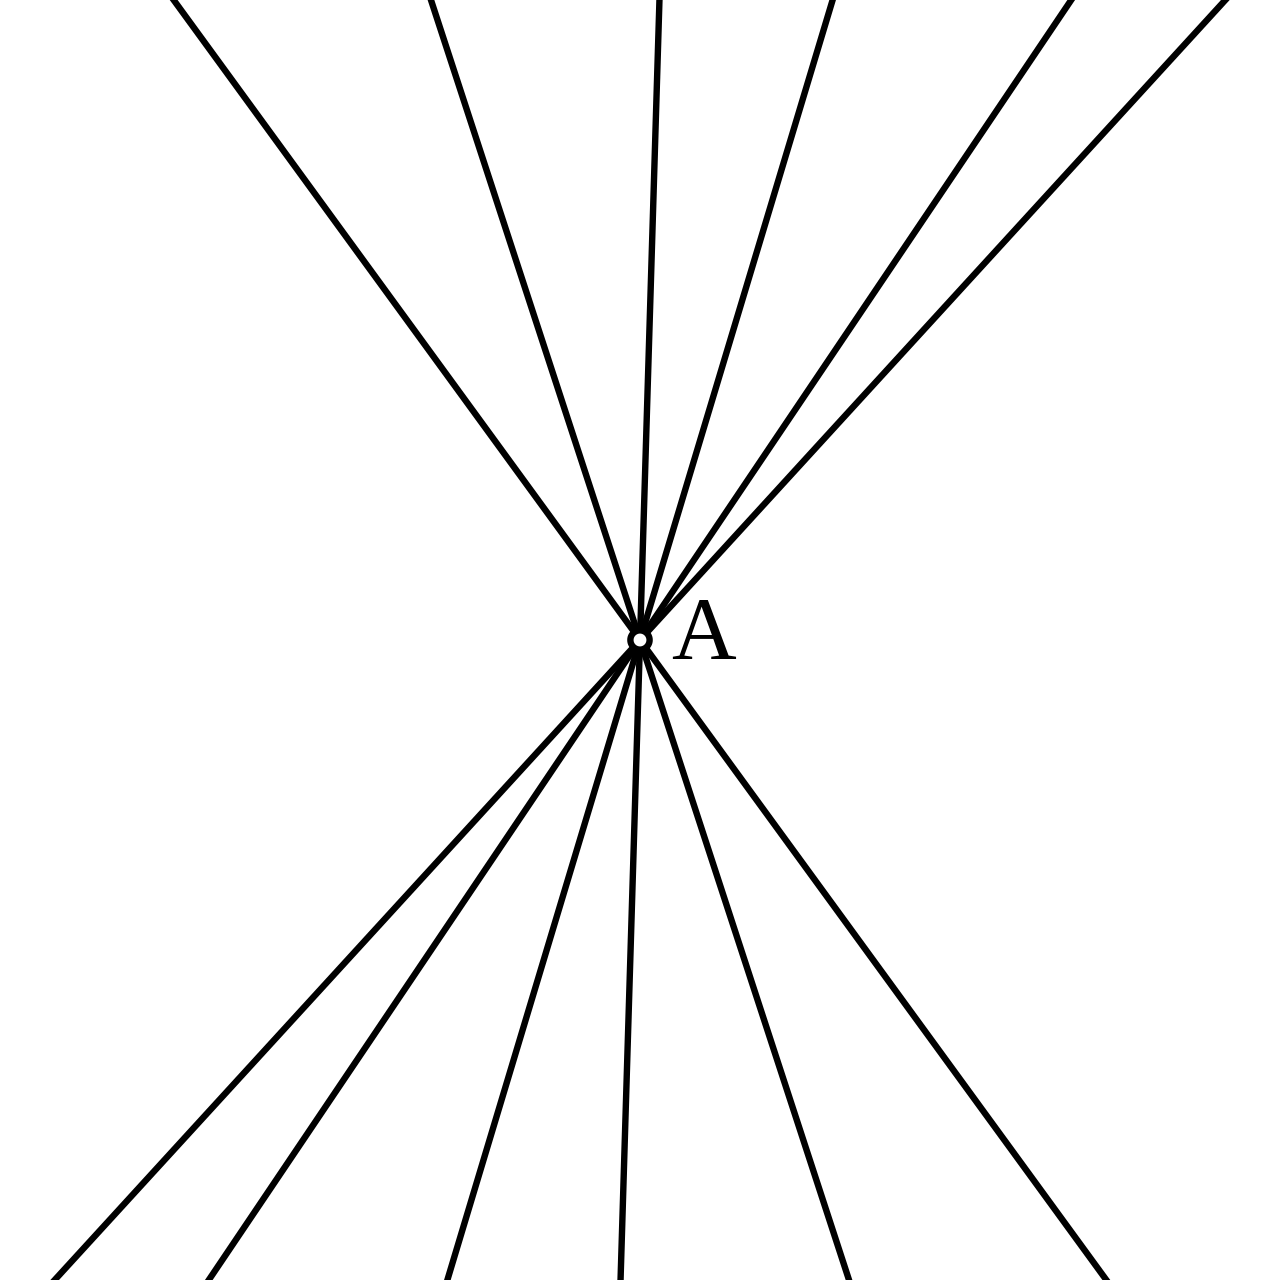
\includegraphics[width=0.4\textwidth]{pencil.png}
		\caption*{Some lines in the pencil through $A$}
	\end{figure}
	If $\codim X^*=1$, then $X^*$ is a hypersurface in $\P(V^*)$, so it is given as zero locus of some reduced homogeneous polynomial $P_X$ of degree $d^*$, which is defined up to multiplication by an invertible constant. This poylnomial $P_X$ is known as \textit{\textbf{discriminant}} of $X$. Reason:

\end{proof}

\subsection{June 10, some exercises}\label{ssec:June 10, some exercises}

\begin{exercise}[Some part of weak Lefschetz]
	Let $X\subset \C\mathbb{P}^N$ be a smooth projective variety of dimension $N$, and $Y$ a smooth hyperplane section. If $U=X\backslash Y$ is smooth, then
	\[H_k(Y,\Z)\to H_k(X,\Z)\]
	is an isomorphism for $k<n-1$ and surjective for $k=n-1$.
\end{exercise}
\begin{exercise}[Some other part of weak Lefschetz]
	\[H^k(X,\C)\overset{i^*}{\to}H^k(Y,\C)\]
	is an isomorphism for $k<n-1$ and injective for  $k=n-1$.
\end{exercise}
\begin{proof}[Solution]
	Notice that for all $\alpha\in H^k(X,\C)$ we have that $i^*\alpha=0\iff\forall\beta\in H^{n-1-k}(Y,\C)$, $\int i^*\alpha\wedge\beta=0$ by Poincar\'e duality. In this case $\alpha=0$. So if  $\alpha\neq 0$ there must exist $\beta\in H^{2(n-1)-k}(Y,\C)$ such that $\int_{[Y]}i^*\alpha\wedge\beta\neq 0$, which means that $i^*\alpha$ is not zero and $i^*$ is injective.

	Notice that by Poincar\'e duality + hard Lefschetz property, we have a perfect pairing in K\"ahler manifolds given by
	\begin{align*}
		 H^k\times H^k &\longrightarrow k \\
		 (\alpha_1,\alpha_2) &\longmapsto ( (\alpha_1,\alpha_2)) = \int_{[X]}\alpha_1\wedge\alpha_2\wedge L^{n-k}_\omega
	.\end{align*}
	And also, for any functional $\lambda:H^k(X)\to k$ there exists $\alpha\in H^k(X)$ such that $\lambda(-)=\int_XL^{n-k}\wedge\alpha\wedge-$.

	We also know that for any $\alpha\in H^k(X)\backslash 0$ there exists $\beta\in H^k(X)$ such that $\int_{[X]}L\wedge L^{n-k-1}\wedge\alpha\wedge\beta\neq 0$.
	\begin{claim}
		$\deg(\gamma\cap\omega\cap[X])=\int_X\omega\wedge\gamma=\int_Yi^*(\gamma)\overset{\text{proj. formula}}{=}\int_{i_*[Y]}=\langle i\in[Y],\gamma\rangle_X=\deg(\gamma\cap i_*[Y])$.	
	\end{claim}

Modulo this true-important-homework claim, we get that

for any $\alpha\neq 0\in H^k(X)\backslash 0\;\exists \beta\in H^k(X)$ such that $\int_{[X]}L\wedge L_x^{n-k-1}\wedge\alpha\wedge\beta\neq 0$, and also this is equal to $\int_{[Y]}L_Y^{n-k-1}\wedge i^*\alpha\wedge i^*\beta$ so I guess there exists $\alpha'\in H^{2(n-1)-k}(Y)$ with $\alpha'=i^*\beta\wedge\omega^{n-k-1}$.

For surjectivity, consider $i^*\alpha\in H^k(Y)$, which is a functional on $H^{2(n-1)-k}(Y)\ni\beta$
\end{proof}

\begin{remark}
	While we struggled a bit with surjectivity, injectivity should be clear.
\end{remark}

\subsection{June 17: Chern connection}\label{sec:June 17: Chern connection}

\begin{enumerate}
	\item Define a \textit{\textbf{connection}} for a given vector bundle $E\to B$ to be a map
		\[\mathcal{A}^0(E)\to\mathcal{A}^1(E)\]
satisfying Leibniz identity that
\[\nabla (f\cdot s)=df\otimes s+f\cdot\nabla s.\]
\item Notice that the difference of two connections $D_1$ and $D_2$ when evaluated on the section $f\cdot s$ differ only by the second term, that is
	 \[(D_1-D_2)(fs)=f(D_1-D_2)s\]
	 which makes it a {\color{magenta}tensor?}
 \item We may generalize this definition to $\mathcal{A}^k(E)\to \mathcal{A}^{k+1}(E)$.
 \item Then we get
	 \[\begin{tikzcd}[column sep=small]
		 \mathcal{A}^{0}(E)\arrow[r,"D"]&\mathcal{A}^{1}(E)\arrow[r,"D"]&\mathcal{A}^2(E)\arrow[r,"D"]&\cdot
	 \end{tikzcd}\]
	 and we define the composition $D\circ D:\mathcal{A}^0(E)\to \mathcal{A}^2(E)$ to be the \textit{\textbf{curvature}}  of this connection, denoted y $F_D\in \mathcal{A}^2\operatorname{End}(E)$.
 \item Now consider $\det(F_D+\lambda1_E)=\sum \lambda^k\omega_K^D$ and call $[\omega^D]:=c_k(E)$ the \textit{\textbf{Chern classes of $E$}}. The first one is $c_1(E)=[\operatorname{tr}(F^D)]$ and the \textit{\textbf{Chern character}} is $\operatorname{ch}(E)=[\operatorname{tr}(e^{FD})$.
 \item Now go to Dolbeault complex. Similarly, we have a map
	 \[\overline{\partial}:\mathcal{A}^0(E)\to\mathcal{A}^{0,1}(E)\]
	 satisfying
	 \[\overline{\partial}(f\cdot s)=\overline{\partial}f\otimes s+f(\overline{\partial}s)\]
	 and extend it to
	 \[\begin{tikzcd}[column sep=small]
		 \mathcal{A}^{0}(E)\arrow[r]&\mathcal{A}^{0,1}(E))\arrow[r]&\mathcal{A}^{0,2}(E)\arrow[r]&\cdots
	 \end{tikzcd}\]
 \item So Leibniz for $D$ implies two Leibniz rules:
	  \begin{enumerate}
	 	\item \[D^0(fs)=\overline{\partial}f\otimes +fD^{0,s}s\]
		\item \[D^{1,0}(fs)=\partial fs+D_{0,1}s\]
	 \end{enumerate}
 \item Fact:
	 \begin{thm}[Some fact]
	 	For any holomorphic vector bundle over a complex manifold there is a natural $(0,1)$-connection.
	 \end{thm}
	 \begin{defn}[Hermitian connection]
	 	
		 Connection $D$ is \textit{\textbf{hermitian}} when
		\[h(s,s)=h(Ds,s)+h(s,Ds).\]
	 \end{defn}
	 Ahora s\'i,
	 \begin{thm}[Chern]
	 	For every hermitian vector bundle $(E,h)$ there exists a unique Hermitian connection $D$ such that
		\[D^{0,1}=\overline{\partial}_E\]
	 \end{thm}
 \item Now take the curvature of the Chern connection. It is a real $(1,1)$-form and then we have the \textit{\textbf{Chern class}}:
	 \[c_1(E):=[\operatorname{tr}(F^D)]\in H^{1,1}(X,\Z)\]Similarly, the
	 \[c_k(E)\in H^{k,k}(X,\C)\cap H^{2k}(X,\Z)\]
\end{enumerate}
\subsubsection{Chern classes axiomatically}\label{ssec:Chern classes axiomatically}
Fix $k=\Z,\R,\C,\ldots$.
\begin{enumerate}
	\item For any topological space $X$ in some nice class and any complex vector bundle $E/X$ we have
		\[c_k(E)\in H^{2k}(X,k)\]
\item \textbf{Functoriality (base change pullback).} We must ask that if $f:Y\to E/X$ 
\[c_k(f^*E)=f^*c_k(E)\]
where $f^*:H^{2k}(X,k)\to H^{2k}(Y,k)$ is the induced map.
\item \textbf{Whittney formula}\[c(E\oplus F)=c(E)\cup c(F)\]
	\[c_k(E\oplus F)\sum_{a+b=k} c_a(E)\smile c_b(F)\]
\item \[c_k(E)=0\quad \text{for } k>\operatorname{rk}E\]
\item \[c_1(\mathcal{O}_{\C\P^1}(1))=[P]\in H^{2}(\C\P^1,k).\]
\end{enumerate}
	
\begin{thm}[Stiefel? Whitney?]
	Such $c_k$ exist and for any $k=\Z,\R,\C,\ldots$ any two are equal.
\end{thm}
\subsubsection{kodaira vanishing}\label{sec:kodaira-vanishing}
Now let's consider the commutator {\color{magenta}anticommutator?}
\[F^D=\{D^{1,0},\overline{\partial}_E\}\]
\begin{remark}
	Recall that for a complex vector bundle $(\mathcal{L},h)$ with $X=\bigcup U_i$ and $\mathcal{L}|_{U_i}=\mathcal{O}|_{U_i}$. {\color{magenta}Then something related to the logarithm of a section that I really didn't understand…}
\end{remark}

Now let's do some Hodge theory on a K\"ahler manifold $(X,g)$.We have the operator
\[\overline{\partial}_E:\Ac^{0,k}(E)\to\mathcal{A}^{0,k+1}(E)\]
and its adjoint
\[-\overline{*}_E\partial\overline{*}_E=\overline{\partial}_E^*:\mathcal{A}^{0,k+1}(E)\to\mathcal{A}^{0,k}(E)\]
and the K\"ahler identities...
\begin{align*}
	[L,d]=0=[L,d]\\
	[L,D^{1,0}]=0\\
	[\Lambda,\overline{\partial}]=i\partial^*\qquad\text{K\"ahler identity} \\
	[\Lambda,\overline{\partial}_E]=i(D^{1,0})^*\qquad\text{Nakano identity}
\end{align*}
And then there is also
\begin{thm}[Hodge theorem]
	In every clas of $H^{p,q}(X,E)$ there is a unique harmonic representative $\alpha\in \mathcal{H}^{p,q}(X,E)$ such that
	\[\overline{\partial}_E\alpha=0\qquad\overline{\partial}_E^*\alpha=0\]
\end{thm}
{\color{magenta}Then some computations using these equations…}

\begin{thm}[Kodaira vanishing]
	If $L$ is positive (there exists $h$ such that $\omega_{L,h}>0$ then
	\[H^{p,q}(X,\mathcal{L})=0\qquad p+q>n=\dim X\]
\end{thm}
\begin{proof}
	From Nakano identity go to some inequalities involving $(F^D\wedge\alpha,\alpha)=?$, back to Lefschetz… \textit{it is not (supposed to be) too complicated.}
\end{proof}

Ok now let's move onto something else. Let $Y\subset X$ be a hyperplane section and $(X,\mathcal{L})$ be such that $(X,\mathcal{L},h)$ is a positive line bundle. Consider two short exact sequences:
\[\begin{tikzcd}
	0\arrow[r]&\mathcal{O}_X(-Y)\arrow[r,hook]&\mathcal{O}_X\arrow[r]&\mathcal{O}_Y\arrow[r]&0
\end{tikzcd}\]
and
\[\begin{tikzcd}
	0\arrow[r]&\mathcal{O}_Y(-Y)\arrow[r]&\Omega_X|_Y\arrow[r]&\Omega_Y\arrow[r]&0
\end{tikzcd}\]
And then take $\Lambda^n$ to get
\[\begin{tikzcd}
	0\arrow[r]&\Omega^{n-1}_Y(-Y)\arrow[r]&\Omega^n_{X|_Y}\arrow[r]&\Omega^n_Y\arrow[r]&0
\end{tikzcd}\]
And then
\[\begin{tikzcd}
	0\arrow[r]&\Omega^n_X(-Y)\arrow[r]&\Omega^n_X\arrow[r]&\Omega^n_X\otimes\mathcal{O}_Y\arrow[r]&0
\end{tikzcd}\]
And then we get some long exact sequences:
\[\begin{tikzcd}[column sep=tiny,row sep=tiny]
	H^{q}(Y,\Omega^p_X|_Y)\arrow[r]&H^{q}(X,\Omega^p_X)\arrow[r]&H^{q}(X,\mathcal{O}_Y\otimes\Omega^p_X)\arrow[r]&H^{q+1}(X,\Omega^p_X(-Y))\arrow[d,equals]\arrow[r]&\cdots\\
				       &&&H^{p,q+1}(X,\mathcal{O}(-Y))\arrow[d,equals]\\
				       &&&H^{n+1-p,n-q}(X,\mathcal{O}(Y))
\end{tikzcd}\]

\subsection{kodaira embedding}\label{sec:June 19}
\begin{coro}[3]
	In a compact space, if you have any line bundle $(E,h)$, if $L>0$ is a positive bundle, then you can twist $E$ by a sufficiently big power of $L$ to make it positive. In symbols, $\exists N$ such that $\forall k\geq N$
	\[E\otimes L^k>0.\]
\end{coro}
Let's write just for the pleasure of writing that for a compact complex manifold $X$,
\begin{thm}[kodaira vanishing]
	If $L>0$, $H^{p,q}(X,L)=0$ for $p+q>n$.
\end{thm}
and that
\begin{thm}[serre-duality version 2.3]
	$H^{p',q'}(X,L^\vee)=0$ for $p'+q'=0$.
\end{thm}
and guess what
\begin{thm}[serre vanishing]
	$L>0$, $\forall E \exists N$ such tat $H^{p,q}(X,E\otimes L^k)=0$ for all $q>0, \forall k\geq N$.
\end{thm}
And now,
\begin{thm}[kodaira embedding]
	For $X$ compact, $\operatorname{Pic}X\ni L$ is ample iff $L>0$.
\end{thm}
\begin{proof}
	Let $L>0$ and lets find some $k$ such that
	\[|L|^k:X\to\P^n\]
	\begin{enumerate}
		\item $\Gamma(X,L^{\otimes })$
		\item L.S. $|L^k|$ is base point free, $\operatorname{bs}L^k=\0$.
		\item $f:X\to \P^n=\P(\Gamma(S,L^k))$  is
			\begin{enumerate}
				\item injective
				\item $\forall x\in X$  $df|_X:T_xX\to T_{fx}\P$ is injective.
			\end{enumerate}
			
	\end{enumerate}
	Now

\end{proof}

\paragraph{Step 1} $\forall x\in X$ there exists $k$ such that $\notin \operatorname{Bs}L^k$ for $k\geq n$ and $s \in \Gamma(X,L^k)$ with $s(x)\neq 0$.

Remember that we always have

\[\begin{tikzcd}
	0\arrow[r]&\mathcal{I}_X\arrow[r,hook]&\mathcal{O}_X\arrow[r]&\mathcal{O}_X\arrow[r]&0
\end{tikzcd}\]
Multiplying by $\bigoplus L^k$ we get
\[\begin{tikzcd}
	0\arrow[r]&\mathcal{I}_X\otimes L^{\otimes k}\arrow[r]&L^{\otimes k}\arrow[r]&(L^{\otimes k})\otimes \mathcal{O}_X\arrow[r]&0
\end{tikzcd}\]
And then pass to the long one
\[\begin{tikzcd}[column sep=small]
	0\arrow[r]&\Gamma(X,\mathcal{I}_X\otimes L^{\otimes (k)})\arrow[r]&\Gamma(X,L^{\otimes k})\arrow[r]&\Gamma(X,\mathcal{O}_X\otimes L^{\otimes k})\arrow[r]&H^{1}(X,\mathcal{I}_X\otimes L^{\otimes k})\arrow[r]&\cdots
\end{tikzcd}\]
Then is the part of the blow-up:
\[\begin{tikzcd}[column sep=small]
	\P^{n-1}=\P(T_xX)=E\arrow[r,hook,"i_E"]\arrow[d,"\pi"]&\operatorname{Bl}_xX=\overline{X}\arrow[d,"G"]\\
	\bullet\arrow[r]&X
\end{tikzcd}\]
{\color{blue}[Unsure of the ending…]}

\section{June 24}\label{sec:June 24}
E for \textbf{exceptional divisor}, Z for \textbf{zenter=center}, X for a manifold and $\widetilde{X}$ for the total space.
\[\begin{tikzcd}
	E\arrow[r,hook]\arrow[d,"\pi",swap]&\widetilde{X}\arrow[d,"\sigma"]\\
	Z\arrow[r,hook]& X
\end{tikzcd}\]

\section{Chow}\label{sec:Chow}
Start from a variety $X^{(d)}\subset \P^{n}$ produce an effective divisor  $C_{X}\subset \operatorname{Gr}(n-d-1,n+1) $. {\color{blue}Using universal subbundle?}

\begin{quotation}
	"Picard group is cyclic generated by $\mathcal{O}(n)"$
\end{quotation}

\section{Last lecture!}\label{sec:Last lecture!}
What is an elliptic curve?

\end{document}
